% Options for packages loaded elsewhere
\PassOptionsToPackage{unicode}{hyperref}
\PassOptionsToPackage{hyphens}{url}
\PassOptionsToPackage{dvipsnames,svgnames,x11names}{xcolor}
%
\documentclass[
  letterpaper,
  DIV=11,
  numbers=noendperiod]{scrreprt}
\usepackage{amsmath,amssymb}
\usepackage{lmodern}
\usepackage{iftex}
\ifPDFTeX
  \usepackage[T1]{fontenc}
  \usepackage[utf8]{inputenc}
  \usepackage{textcomp} % provide euro and other symbols
\else % if luatex or xetex
  \usepackage{unicode-math}
  \defaultfontfeatures{Scale=MatchLowercase}
  \defaultfontfeatures[\rmfamily]{Ligatures=TeX,Scale=1}
\fi
% Use upquote if available, for straight quotes in verbatim environments
\IfFileExists{upquote.sty}{\usepackage{upquote}}{}
\IfFileExists{microtype.sty}{% use microtype if available
  \usepackage[]{microtype}
  \UseMicrotypeSet[protrusion]{basicmath} % disable protrusion for tt fonts
}{}
\makeatletter
\@ifundefined{KOMAClassName}{% if non-KOMA class
  \IfFileExists{parskip.sty}{%
    \usepackage{parskip}
  }{% else
    \setlength{\parindent}{0pt}
    \setlength{\parskip}{6pt plus 2pt minus 1pt}}
}{% if KOMA class
  \KOMAoptions{parskip=half}}
\makeatother
\usepackage{xcolor}
\IfFileExists{xurl.sty}{\usepackage{xurl}}{} % add URL line breaks if available
\IfFileExists{bookmark.sty}{\usepackage{bookmark}}{\usepackage{hyperref}}
\hypersetup{
  pdftitle={Model Exploration},
  pdfauthor={Jane Doe},
  colorlinks=true,
  linkcolor={blue},
  filecolor={Maroon},
  citecolor={Blue},
  urlcolor={Blue},
  pdfcreator={LaTeX via pandoc}}
\urlstyle{same} % disable monospaced font for URLs
\usepackage{color}
\usepackage{fancyvrb}
\newcommand{\VerbBar}{|}
\newcommand{\VERB}{\Verb[commandchars=\\\{\}]}
\DefineVerbatimEnvironment{Highlighting}{Verbatim}{commandchars=\\\{\}}
% Add ',fontsize=\small' for more characters per line
\usepackage{framed}
\definecolor{shadecolor}{RGB}{241,243,245}
\newenvironment{Shaded}{\begin{snugshade}}{\end{snugshade}}
\newcommand{\AlertTok}[1]{\textcolor[rgb]{0.68,0.00,0.00}{#1}}
\newcommand{\AnnotationTok}[1]{\textcolor[rgb]{0.37,0.37,0.37}{#1}}
\newcommand{\AttributeTok}[1]{\textcolor[rgb]{0.00,0.48,0.65}{#1}}
\newcommand{\BaseNTok}[1]{\textcolor[rgb]{0.68,0.00,0.00}{#1}}
\newcommand{\BuiltInTok}[1]{\textcolor[rgb]{0.00,0.48,0.65}{#1}}
\newcommand{\CharTok}[1]{\textcolor[rgb]{0.13,0.47,0.30}{#1}}
\newcommand{\CommentTok}[1]{\textcolor[rgb]{0.37,0.37,0.37}{#1}}
\newcommand{\CommentVarTok}[1]{\textcolor[rgb]{0.37,0.37,0.37}{\textit{#1}}}
\newcommand{\ConstantTok}[1]{\textcolor[rgb]{0.56,0.35,0.01}{#1}}
\newcommand{\ControlFlowTok}[1]{\textcolor[rgb]{0.00,0.48,0.65}{#1}}
\newcommand{\DataTypeTok}[1]{\textcolor[rgb]{0.68,0.00,0.00}{#1}}
\newcommand{\DecValTok}[1]{\textcolor[rgb]{0.68,0.00,0.00}{#1}}
\newcommand{\DocumentationTok}[1]{\textcolor[rgb]{0.37,0.37,0.37}{\textit{#1}}}
\newcommand{\ErrorTok}[1]{\textcolor[rgb]{0.68,0.00,0.00}{#1}}
\newcommand{\ExtensionTok}[1]{\textcolor[rgb]{0.00,0.48,0.65}{#1}}
\newcommand{\FloatTok}[1]{\textcolor[rgb]{0.68,0.00,0.00}{#1}}
\newcommand{\FunctionTok}[1]{\textcolor[rgb]{0.28,0.35,0.67}{#1}}
\newcommand{\ImportTok}[1]{\textcolor[rgb]{0.00,0.48,0.65}{#1}}
\newcommand{\InformationTok}[1]{\textcolor[rgb]{0.37,0.37,0.37}{#1}}
\newcommand{\KeywordTok}[1]{\textcolor[rgb]{0.00,0.48,0.65}{#1}}
\newcommand{\NormalTok}[1]{\textcolor[rgb]{0.00,0.48,0.65}{#1}}
\newcommand{\OperatorTok}[1]{\textcolor[rgb]{0.37,0.37,0.37}{#1}}
\newcommand{\OtherTok}[1]{\textcolor[rgb]{0.00,0.48,0.65}{#1}}
\newcommand{\PreprocessorTok}[1]{\textcolor[rgb]{0.68,0.00,0.00}{#1}}
\newcommand{\RegionMarkerTok}[1]{\textcolor[rgb]{0.00,0.48,0.65}{#1}}
\newcommand{\SpecialCharTok}[1]{\textcolor[rgb]{0.37,0.37,0.37}{#1}}
\newcommand{\SpecialStringTok}[1]{\textcolor[rgb]{0.13,0.47,0.30}{#1}}
\newcommand{\StringTok}[1]{\textcolor[rgb]{0.13,0.47,0.30}{#1}}
\newcommand{\VariableTok}[1]{\textcolor[rgb]{0.07,0.07,0.07}{#1}}
\newcommand{\VerbatimStringTok}[1]{\textcolor[rgb]{0.13,0.47,0.30}{#1}}
\newcommand{\WarningTok}[1]{\textcolor[rgb]{0.37,0.37,0.37}{\textit{#1}}}
\usepackage{longtable,booktabs,array}
\usepackage{calc} % for calculating minipage widths
% Correct order of tables after \paragraph or \subparagraph
\usepackage{etoolbox}
\makeatletter
\patchcmd\longtable{\par}{\if@noskipsec\mbox{}\fi\par}{}{}
\makeatother
% Allow footnotes in longtable head/foot
\IfFileExists{footnotehyper.sty}{\usepackage{footnotehyper}}{\usepackage{footnote}}
\makesavenoteenv{longtable}
\usepackage{graphicx}
\makeatletter
\def\maxwidth{\ifdim\Gin@nat@width>\linewidth\linewidth\else\Gin@nat@width\fi}
\def\maxheight{\ifdim\Gin@nat@height>\textheight\textheight\else\Gin@nat@height\fi}
\makeatother
% Scale images if necessary, so that they will not overflow the page
% margins by default, and it is still possible to overwrite the defaults
% using explicit options in \includegraphics[width, height, ...]{}
\setkeys{Gin}{width=\maxwidth,height=\maxheight,keepaspectratio}
% Set default figure placement to htbp
\makeatletter
\def\fps@figure{htbp}
\makeatother
\setlength{\emergencystretch}{3em} % prevent overfull lines
\providecommand{\tightlist}{%
  \setlength{\itemsep}{0pt}\setlength{\parskip}{0pt}}
\setcounter{secnumdepth}{5}
\KOMAoption{captions}{tableheading}
\makeatletter
\makeatother
\makeatletter
\@ifpackageloaded{caption}{}{\usepackage{caption}}
\AtBeginDocument{%
\renewcommand*\contentsname{Table of contents}
\renewcommand*\listfigurename{List of Figures}
\renewcommand*\listtablename{List of Tables}
\renewcommand*\figurename{Figure}
\renewcommand*\tablename{Table}
}
\@ifpackageloaded{float}{}{\usepackage{float}}
\floatstyle{ruled}
\@ifundefined{c@chapter}{\newfloat{codelisting}{h}{lop}}{\newfloat{codelisting}{h}{lop}[chapter]}
\floatname{codelisting}{Listing}
\newcommand*\listoflistings{\listof{codelisting}{List of Listings}}
\makeatother
\makeatletter
\@ifpackageloaded{caption}{}{\usepackage{caption}}
\@ifpackageloaded{subcaption}{}{\usepackage{subcaption}}
\makeatother
\makeatletter
\makeatother
\ifLuaTeX
  \usepackage{selnolig}  % disable illegal ligatures
\fi

\title{Model Exploration}
\author{Jane Doe}
\date{\texttt{r\ Sys.Date()}}

\begin{document}
\maketitle

\renewcommand*\contentsname{Table of contents}
{
\hypersetup{linkcolor=}
\setcounter{tocdepth}{2}
\tableofcontents
}
\hypertarget{preface}{%
\chapter*{Preface}\label{preface}}
\addcontentsline{toc}{chapter}{Preface}

This is a Quarto book.

To learn more about Quarto books visit
\url{https://quarto.org/docs/books}.

\begin{Shaded}
\begin{Highlighting}[]
\DecValTok{1} \SpecialCharTok{+} \DecValTok{1}
\end{Highlighting}
\end{Shaded}

\begin{verbatim}
[1] 2
\end{verbatim}

\hypertarget{quantifying-art-historical-narratives-chapter-1}{%
\chapter{Quantifying Art Historical Narratives, Chapter
1}\label{quantifying-art-historical-narratives-chapter-1}}

\hypertarget{abstract}{%
\section{Abstract}\label{abstract}}

My project surveys the development of \emph{Janson's History of Art}
across its eight editions as well as \emph{Gardner's Art Through the
Ages} through its sixteen editions, looking particularly at the change
in artist demographic through time. Additionally, this paper
investigates which external variables such as artist gender, ethnicity,
race, nationality, number of exhibitions at the Museum of Modern Art and
The Whitney, and number of publications on WorldCat, if any, help
predict the magnitude of an artist's inclusion in art history survey
texts. I conduct data analysis to assess the demographic representation
of artists through editions of \emph{Janson's History of Art} and
\emph{Gardner's Art Through the Ages}, a proxy for the art history
survey. I compare artist demographics through editions of Janson and
Gardner. My findings indicate that coverage of minority artists (defined
as non-white and/or Hispanic or Latinx and/or female) increases across
editions of \emph{Janson's History of Art} and \emph{Gardner's Art
Through the Ages}, but remains negligible compared to white male
non-Hispanic or Latinx artists. Moreover, in \emph{Janson's History of
Art} through all editions, the percentage of artists who are white is
98.04\%, the percentage of artists that are male is 92.47\%, and the
percentage of artists that are not Hispanic or Latinx is 92.04\%. In
\emph{Gardner's Art Through the Ages}, through all editions, the
percentage of artists who are white is 92.76\%, the percentage of
artists that are male is 90.47\%, and the percentage of artists that are
not Hispanic or Latinx is 90.94\%. Both texts display a narrative of the
history of art as being predominantly white, male, non-Hispanic or
Latinx. Regarding nationality, in Janson, 81.52\% of the artists are
American, British, French, German, and Spanish, which is very similar to
Gardner's 79.30\% of those five same nationalities. I have chosen to run
a linear mixed-effects model with a random effect of
\texttt{artist\_name}, to infer the magnitude of the ratio of space
given to a particular artist, \texttt{space\_ratio\_per\_page\_total} in
\emph{Janson's History of Art} and \emph{Gardner's Art Through the
Ages,} using the potential predictor variables: \texttt{artist\_race},
\texttt{artist\_gender} , \texttt{artist\_ethnicity} ,
\texttt{artist\_nationality\_other} , \texttt{moma\_count\_to\_date} ,
\texttt{whitney\_count\_to\_date}, and the two interaction variables of
\texttt{artist\_gender*moma\_count\_to\_date} and
\texttt{artist\_nationality\_other*moma\_count\_to\_date}. With a log
transformation applied to the outcome variable,
\texttt{space\_ratio\_per\_page\_total} as it is heavily right-skewed,
my linear mixed-effects model yields a conditional r squared of 53.23\%.
Such denotes that 53.21\% total variance of the outcome variable,
\texttt{space\_ratio\_per\_page\_total} is explained through the fixed
predictor variables as listed above and the random effect of
\texttt{artist\_name}.

JEL Numbers: C80, Y10, Z11

Key Words: Cultural Economics, Art History, Statistics, Historiography,
Data Collection Methodology, Linear Mixed-Effects Modeling.

Data Preparation:

\hypertarget{introduction-and-context}{%
\section{Introduction and Context}\label{introduction-and-context}}

\hypertarget{inspiration-for-research}{%
\subsection{Inspiration for Research:}\label{inspiration-for-research}}

Heading into the second semester of my junior year, I scheduled a zoom
meeting with my now undergraduate thesis advisor, Prof.~Hans van
Miegroet, to ask a few questions about my aspirations after college. He
had been my professor for his course, ``History of Art Markets,'' a
learning experience at Duke that has permanently altered my worldview.
The meeting began with me expressing my enjoyment of the course, and the
appreciation of the discussion of transparency in the buying and selling
of art. I asked his opinion of whether I should stick to studying
architectural history with hopes of going to architecture school, or
pivot to do further research under him in his graduate course, ``Arts
and Markets'' that I had enrolled in for that Spring. Towards the end of
the meeting, he asked me what I found most interesting about art, to
which I replied, ``Ever since I took my first Art History course, I've
always been curious as to why I am introduced to the works I am. Who is
choosing what I study versus what I don't study?'' I explained to him. I
had initially learned the story of art through Marilyn Stokstad's,
\emph{Art History} my final year of high school. At the end of that
school year, I inquired to my teacher, Carolyn Paczkowska, in a class
discussion, ``Why are we studying the works that we have?'' The class
discussed gatekeepers of art and information and later ended in the
conclusion of uncertainty. Prof.~van Miegroet looked at me through the
computer screen and stated I had found my research question for my
Undergraduate Honors Thesis, that I had found my why.

My research began solely looking at how art history textbooks changed
through time, then developed into looking at using a linear mixed-effect
model with a log transformation on my outcome variable to infer which
external variables would if at all work to predict the magnitude of
space (of text and of the figure of their work or works) given to an
artist in a given book.

\hypertarget{why-gardners-art-through-the-ages}{%
\subsection{\texorpdfstring{Why \emph{Gardner's Art Through the
Ages:}}{Why Gardner's Art Through the Ages:}}\label{why-gardners-art-through-the-ages}}

\hypertarget{discourse-of-authorship}{%
\subsubsection{Discourse of Authorship:}\label{discourse-of-authorship}}

\hypertarget{literature-review}{%
\subsubsection{Literature Review:}\label{literature-review}}

\textbf{(}Discourse of dominance through time of the text, find and add
sources and if available sales information through time)

REACH OUT FOR SALES DATA TO PUBLISHERS

Britannica

\begin{itemize}
\tightlist
\item
  The lack of a
  \href{https://www.merriam-webster.com/dictionary/comprehensive}{comprehensive}
  single-volume textbook on art history prompted Gardner to write one
  herself, and the resulting Art Through the Ages (1926) far surpassed
  other available works in readability, breadth of coverage, and wealth
  of illustration. It remained a widely used text for decades. In 1932
  she published Understanding the Arts, aimed at a wide general
  audience. A second edition of Art Through the Ages, greatly expanded,
  appeared in 1936; \textbf{the first two editions sold more than
  260,000 copies.} Gardner had been named an assistant professor in the
  Art Institute school in 1929, and in 1933 she became a professor and
  head of the department of art history. She retired from the Art
  Institute school in 1943. Despite declining health she managed to
  complete work on the manuscript of a third edition of Art Through the
  Ages (published in 1948).
\end{itemize}

Sources Found to Looking Into:

\begin{itemize}
\tightlist
\item
  Franciscono, Marcel.

  \begin{enumerate}
  \def\labelenumi{\arabic{enumi}.}
  \setcounter{enumi}{1976}
  \tightlist
  \item
    ``History, Textbooks, and Art: Reflections on a Half Century of
    Helen Gardner's''Art through the Ages''.'' Critical Inquiry 4 (2)
    (Winter): 285. https://login.proxy.lib.duke.edu/login?u
    rl=https://www.proquest.com/scholarly-journals/history-textbooks-art-reflections-on-half-century/docview/1297337757/se-2?a
    ccountid=10598.
  \end{enumerate}
\item
  Jaffee, Barbara. ``9.''Gardner'' Variety Formalism: Helen Gardner and
  Art through the Ages'' In Partisan Canons edited by Anna Brzyski,
  203-224. New York, USA: Duke University Press, 2007.
  https://doi.org/10.1515/9780822390374-010.
\end{itemize}

\textbf{Table 1:} Edition Number, Year of Publication, Title,
Authorship, and Publisher Over Time of All Cataloged Editions of
Gardner's Art Through the Ages.

\begin{longtable}[]{@{}
  >{\raggedright\arraybackslash}p{(\columnwidth - 8\tabcolsep) * \real{0.0458}}
  >{\raggedright\arraybackslash}p{(\columnwidth - 8\tabcolsep) * \real{0.0840}}
  >{\raggedright\arraybackslash}p{(\columnwidth - 8\tabcolsep) * \real{0.3740}}
  >{\raggedright\arraybackslash}p{(\columnwidth - 8\tabcolsep) * \real{0.2748}}
  >{\raggedright\arraybackslash}p{(\columnwidth - 8\tabcolsep) * \real{0.2214}}@{}}
\toprule
\begin{minipage}[b]{\linewidth}\raggedright
Edition
\end{minipage} & \begin{minipage}[b]{\linewidth}\raggedright
Year of Publication
\end{minipage} & \begin{minipage}[b]{\linewidth}\raggedright
Author(s)
\end{minipage} & \begin{minipage}[b]{\linewidth}\raggedright
Title
\end{minipage} & \begin{minipage}[b]{\linewidth}\raggedright
Publisher (as listed per Edition)
\end{minipage} \\
\midrule
\endhead
1 & 1926 & Helen Gardner & Art through the ages; an introduction to its
history and significance & New York, Brace, Harcourt \\
2 & 1936 & Helen Gardner & Art through the ages; an introduction to its
history and significance & New York, Brace, Harcourt \\
3 & 1948 & Helen Gardner & Art through the ages & New York, Brace,
Harcourt \\
4 & 1959 & Helen Gardner; revised by Sumner M. Crosby and the Dept. of
the History of Art, Yale University & Art through the ages & New York,
Harcourt, Brace \\
5 & 1970 & Revised by Horst de la Croix, Richard G. Tansey & Gardner's
art through the ages & New York, Harcourt, Brace \\
6 & 1975 & Helen Gardner; revised by Horst de la Croix, Richard G.
Tansey & Gardner's art through the ages & New York: Harcourt Brace
Jovanovich \\
7 & 1980 & Helen Gardner; revised by Horst de la Croix, Richard G.
Tansey & Gardner's art through the ages & Harcourt Brace Jovanovich, New
York \\
8 & 1986 & Horst de la Croix, Richard G. Tansey & Gardner's art through
the ages & Harcourt Brace Jovanovich, San Diego, CA \\
9 & 1991 & Horst de la Croix, Richard G. Tansey, Diane Kirkpatrick &
Gardner's art through the ages & San Diego: Harcourt Brace Jovanovich \\
10 & 1996 & Richard G. Tansey, Fred S. Kleiner & Gardern's art through
the ages & Fort Worth, TX: Harcourt Brace \\
11 & 2001 & Fred S. Kleiner, Christin J. Mamiya, Richard G. Tansey &
Gardner's art through the ages & Fort Worth TX: Harcourt College
Publishers \\
12 & 2005 & Fred S. Kleiner, Christin J. Mamiya & Gardner's art through
the ages & Thomson/Wadsworth, Belmont, CA \\
13 & 2009 & Fred S. Kleiner & Gardner's art through the ages: a global
history & Boston, Thomson/Wadsworth \\
14 & 2013 & Fred S. Kleiner & Gardner's art through the ages: a global
history & Australia ; United States : Wadsworth, Cengage Learning \\
15 & 2016 & Fred S. Kleiner & Gardner's art through the ages: a global
history & Boston, MA : Cengage Learning \\
16 & 2020 & Fred S. Kleiner & Gardner's art through the ages: a global
history & Boston, MA, US : Cengage Learning \\
\bottomrule
\end{longtable}

\textbf{Table 4:} Authors of Gardner's Art Through the Ages: NEEDS TO BE
ADDED

\hypertarget{why-jansons-history-of-art}{%
\subsection{\texorpdfstring{Why \emph{Janson's History of
Art}:}{Why Janson's History of Art:}}\label{why-jansons-history-of-art}}

Such a text is claimed to be the most influential art history survey
through time by myriad art historians such as Jeffery Wiedman, Zoë
Ingalls, John Russell, Alexandra Peers, Elizabeth Sears and Charlotte
Schoell-Glass to name a few. Alexandra Peers in her publication for
ARTnews.com in February of 2006, claims that ``it was Janson who, more
than any other art historian, pioneers the `in and out' celebrity model
of art history. There were artists who matter, he argued, and those who
didn't.''\footnote{Alexandra Peers, ``Canon Fodder,'' Artnews.com,
  (February 1, 2006),
  https://www.artnews.com/art-news/news/canon-fodder-135/.} Janson's
formation of his history of art is not only arguably the most dominant
art history survey over time, but also he holds a reputation of being a
gatekeeper of art history. He states at the end of his introduction in
the first and second editions that after having read his text, one
``shall have joined the active minority that participates directly in
shaping the course of art in our time.''\footnote{H. W. Janson and Dora
  Jane Janson, (1963),~ History of Art: A Survey of the Major Visual
  Arts from the Dawn of History to the Present Day, First Edition,
  Second Printing, New York: Harry N. Abrams: 17.} He recognizes his
role as an individual who shapes the narrative of the history of art,
while convincing the reader that after having read his text, one has the
agency to be a gatekeeper alongside him . Such agency is only granted
once one understands his digestion of the most important works and
artists through time .

It would be most comprehensive if we were to have access to the total
number of sales per edition of Janson's History of Art, to use as
tangible data to show the relevance and importance of the text through
time. Both publishers, Harry N. Abrams and Prentice-Hall (now Pearson
Prentice-Hall) have declined sharing sales information in the aggregate.
By leafing through various scholarly publications, there is imperfect
data of sale information worth noting when discussing the dominance of
Janson's History of Art through time. The text was at its height of
sales between when it was initially released in 1962 through H. W.
``Peter'' Janson's death in 1982 (refer to Table 1 for complete
information of each edition). Art historian, Patricia Hills cites in her
publication in Artforum, ``in 1973 the Janson text had 46\% of the
market, while Gardner's 5th edition had 24\%, followed by Gombrich's,
8.5\%, Cleaver with 3\% and miscellaneous `other' with
18.5\%.''\footnote{Market Research Report on Introductory Art History,
  dated March 15, 1972, prepared for McGraw-Hill College Textbook
  Division and Follow-up Report, dated Spring, 1973. Citation from
  Patricia Hills, ``Art History Textbooks: The Hidden Persuaders,''
  Artforum, (Summer 1976),
  https://www.artforum.com/print/197606/art-history-textbooks-the-hidden-persuaders-69128.}
At the time such a report had been made, the first edition (1962), the
first edition revised and enlarged (1969) had been released.
Additionally, it was written by John Russell of the New York Times in
October of 1982 that ``well over two million copies have been
sold.''\footnote{John Russell, ``Prof H. W Janson is Dead at 68; Wrote
  Best-Selling `History of Art,'\,'' The New York Times, (October 3,
  1982),
  https://www.nytimes.com/1982/10/03/nyregion/prof-h-w-Janson-is-dead-at-68
  -wrote-best-selling-history-of-art.html.} Russell does not specify
whether these sales numbers are solely the first edition of Janson's
History of Art, or the first edition as well as the first edition
revised and enlarged and the second edition (1977) . He also added that
the text had been ``translated in 14 languages and is widely regarded as
both an essential teaching instrument and a book that can be read and
looked at with continuous enjoyment.''\footnote{John Russell, ``Prof H.
  W Janson is Dead at 68; Wrote Best-Selling `History of Art,'\,'' The
  New York Times, (October 3, 1982),
  https://www.nytimes.com/1982/10/03/nyregion/prof-h-w-Janson-is-dead-at-68
  -wrote-best-selling-history-of-art.html.} Here, Russell perpetuates
the significance of Janson's survey, as well as providing information
about the breadth of Janson's text, reaching more than solely
English-reading audience s.

Conversely, Zoë Ingalls in a publication in August of 1995 discussing
Janson's relevance through time, cites that ``the first edition sold
more than a million copies.''\footnote{Zoë Ingalls, ``A Son Revises His
  Father's Classic Art-History Textbook,'' The Chronicle of Higher
  Education, (August 11, 1995),
  https://www.chronicle.com/article/a-son-revises-his-fathers-classic-
  art-history-textbook/.} Though there are informational discrepancies,
it is clear that Janson's History of Art was prolific as a survey text
of art for over 20 years. The narrative remained significant from the
third (1986) through the fifth edition (1995), which were all revised by
Anthony ``Tony'' F. Janson, son of Peter and Dora Jane. Ingalls states
that ``the fourth edition, published in 1991, sold 21,000 copies the
first year and an average of 11,000 copies a year in the past four
years. The new fifth edition, has sold more than 13,000 copies since its
March release.''\footnote{Zoë Ingalls, ``A Son Revises His Father's
  Classic Art-History Textbook,'' The Chronicle of Higher Education,
  (August 11, 1995),
  https://www.chronicle.com/article/a-son-revises-his-fathers-classic-
  art-history-textbook/.} She continues, ``Although its sales have been
eclipsed over the last 10 years by another perennial favorite, R.H.
Gardner's Art Through the Ages, Janson is still the standard in many
people's minds.''\footnote{Zoë Ingalls, ``A Son Revises His Father's
  Classic Art-History Textbook,'' The Chronicle of Higher Education,
  (August 11, 1995),
  https://www.chronicle.com/article/a-son-revises-his-fathers-classic-
  art-history-textbook/.} Notably, she does not mention any total sales
information about Gardner's survey text, just that over the past decade
(1985-1995), its sales trumped that of Janson' s.

After the sixth edition (2001) and the sixth edition revised (2004) the
last with authorship by Tony Janson, Harry N. Abrams and Prentice Hall
were unsatisfied by the total sales, as well as the overall structure
and content of the text as they were criticized for having lost touch
with young readers.\footnote{Alexandra Peers, ``Canon Fodder.''} At the
same moment, Harry N. Abrams sold all rights to the newly formed Pearson
Prentice Hall, who recruited new authorship of six various art
historians across the United States: Penelope J. E. Davies, Walter B.
Denny, Frima Fox Hofrichter, Joseph Jacobs, Ann M. Roberts, and David L.
Simon (refer to Table 2). Such change was received negatively by art
historians, which is reflected in the text's further decline in sales.
\footnote{Jeffrey Weidman, ``Many Are Culled but Few Are Chosen:
  Janson's History of Art, Its Reception, Emulators, Legacy, and Current
  Demise.'' Journal of Scholarly Publishing 38, no. 2 (January 2007):
  96. https://muse.jhu.edu/article/209994/pdf.} It has been estimated by
Bookauthority.com (a cite whose source for this information is very
unclear) that the eighth edition revised, published in 2015 has had
2,000 total copies sold, while competing art historical narratives such
as Marilyn Stokstad and Micheal W. Cothren's History of Art Vol . 1 has
had an estimated 10,000 copies sold since its release in 2017
.\footnote{``100 Best-Selling Art HIstory Books of All Time,'' Book
  Authority,
  https://bookauthority.org/books/best-selling-art-history-books.} Such
has left Janson's History of Art as a minor player in art historical
narratives today.

\textbf{Table 2:} Edition Number, Year of Publication, Title,
Authorship, and Publisher Over Time of All Cataloged Editions of
Janson's History of Art.

\begin{longtable}[]{@{}
  >{\raggedright\arraybackslash}p{(\columnwidth - 8\tabcolsep) * \real{0.0785}}
  >{\raggedright\arraybackslash}p{(\columnwidth - 8\tabcolsep) * \real{0.0640}}
  >{\raggedright\arraybackslash}p{(\columnwidth - 8\tabcolsep) * \real{0.3198}}
  >{\raggedright\arraybackslash}p{(\columnwidth - 8\tabcolsep) * \real{0.2791}}
  >{\raggedright\arraybackslash}p{(\columnwidth - 8\tabcolsep) * \real{0.2587}}@{}}
\toprule
\begin{minipage}[b]{\linewidth}\raggedright
Edition Number
\end{minipage} & \begin{minipage}[b]{\linewidth}\raggedright
Year of Publication
\end{minipage} & \begin{minipage}[b]{\linewidth}\raggedright
Authors
\end{minipage} & \begin{minipage}[b]{\linewidth}\raggedright
Title
\end{minipage} & \begin{minipage}[b]{\linewidth}\raggedright
Publisher (as listed per Edition)\footnote{There are discrepancies
  through the first and sixth editions of only Harry N. Abrams being
  listed as the publisher on the book itself and Harry N. Abrams and
  Prentice-Hall both being listed. Harry N. Abrams was the primary
  publisher through the first sixth editions as Prentice-Hall was their
  distributor.}
\end{minipage} \\
\midrule
\endhead
1 & 1963\footnote{I cataloged the first edition, second printing,
  published in 1963, but the first edition, first printing was published
  in 1962. There is no different between printings.} & H.W. Janson with
Dora Jane Janson\footnote{Dora Jane Janson is only listed upon opening
  the book to the title page. She is not listed anywhere on the exterior
  of the Janson's History of Art across the first edition, second
  printing, first edition (revised and enlarged) fourteenth printing,
  nor the second edition.} & History of Art: A Survey of the Major
Visual Arts from the Dawn of History to the Present Day & Harry N.
Abrams, Inc., New York \\
1 (Revised and Enlarged) & 1969 & H. W. Janson with Dora Jane Janson &
History of Art: A Survey of the Major Visual Arts from the Dawn of
History to the Present Day & Prentice-Hall Inc., Englewood Cliffs, New
Jersey and Harry N. Abrams, Inc., New York. \\
2 & 1977 & H. W. Janson with Dora Jane Janson & History of Art: A Survey
of the Major Visual Arts from the Dawn of History to the Present Day &
Harry N. Abrams, Inc., New York. \\
3 & 1986 & H. W. Janson; Revised and Expanded by Anthony F. Janson &
History of Art & Harry N. Abrams, Inc., New York and Prentice-Hall Inc.,
Englewood Cliffs, New Jersey.~ \\
4 & 1991 & H. W. Janson; Revised and Expanded by Anthony F. Janson &
History of Art & Harry N. Abrams, Inc., New York. \\
5 & 1995 & H. W. Janson; Revised and Expanded by Anthony F. Janson &
History of Art & \begin{minipage}[t]{\linewidth}\raggedright
Harry N. Abrams, Inc., New York.

\hfill\break
\strut
\end{minipage} \\
6 & 2001 & H. W. Janson and Anthony F. Janson & History of Art &
\begin{minipage}[t]{\linewidth}\raggedright
Harry N. Abrams, Inc., New York.

\hfill\break
\strut
\end{minipage} \\
7 & 2007 & Penelope J. E. Davies, Walter B. Denny, Frima Fox Hofrichter,
Joseph Jacobs, Ann M. Roberts, David L. Simon & Janson's History of Art:
The Western Tradition & Pearson Prentice Hall, Upper Saddle River, New
Jersey. \\
8 & 2011 & Penelope J. E. Davies, Walter B. Denny, Frima Fox Hofrichter,
Joseph Jacobs, Ann M. Roberts, David L. Simon & Janson's History of Art:
The Western Tradition & Pearson Prentice Hall, Upper Saddle River, New
Jersey. \\
\bottomrule
\end{longtable}

\hypertarget{discourse-of-authorship-through-editions}{%
\subsubsection{\texorpdfstring{\textbf{Discourse of Authorship Through
Editions:}}{Discourse of Authorship Through Editions:}}\label{discourse-of-authorship-through-editions}}

The primary author through the first six editions of Janson's History of
Art is Horace Waldemar Janson (1913-1982), colloquially referred to as
Peter. He was born in 1913 in St.~Petersburg, Russia. His parents were
of Swedish and Latvian descent. The family moved to Hamburg, Germany
after the Russian Revolution. Janson studied at Munich and then at the
University in Hamburg where he was a student of Erwin Panofsky, a
prolific art historian known for his contributions to the studies of
symbols and iconography in art. In 1935, at the suggestion of his
advisor, Janson fled Germany under the sponsorship of Alfred Barr,
director of the Museum of Modern Art in New York. Janson studied at
Harvard between 1935 and 1942, completing a PhD in art history. His most
significant professorial position began in 1949, where he was appointed
professor and later chairman of the department of art at New York
University. He remained in such a role for 25 years as he grew the
department's prestige, solidifying its reputation as one of the most
conservative art history programs in the country. A decade later, in
1959, Janson issued a book titled, Key Monuments of the History of Art,
in efforts to aid his undergraduates in their study of art as the
availability of good personal study images were not easily accessible.
Such publication sparked Janson's History of Art released in 1962, a
survey of art written with his wife, Dora Jane Janson.

\hfill\break
Born Dora Jane Heineberg (1916-2002) in Philadelphia in 1916, she shared
a passion for art with Peter. The two met in Cambridge, Massachusetts as
she attended Radcliffe College as an undergraduate student while Janson
was studying at Harvard. Dora Jane Janson worked with her husband on
many publications, but her most notable achievement came in 1971 when
she wrote an exhibition catalog for the Nasher Museum of Art at Duke on
Art Nouveau jewelry, titled From Slave to Siren: The Victorian Woman and
Her Jewelry from Neoclassic to Art Nouveau. Authorship of Janson's
History of Art was handed over to one of the couple's four children,
Anthony F. Janson, after the sudden passing of Peter Janson in 1982.

Anthony Frederick ``Tony'' Janson was born March 30th, 1943 in
St.~Louis, Missouri. The Jansons moved to New York in 1949, and Tony
Janson frequently visited the city's museums as a child and teenager. In
1954, the Jansons spent a year in Europe. In an interview, Tony Janson
describes his attitude upon the family's return to New York as one of ''
total rebellion'' eventually causing his parents to search for a school
that would engage him better academically.\footnote{Anthony Janson,
  interview by Sherman Hayes, University of North Carolina Wilmington
  Archives and Special Collections, (March 15-19, 2007): 11.} Janson
details how he rediscovered a love for learning after enrolling at
Riverdale Country School on a full scholarship, and it is at this time
that he began to study art history. Janson experimented as an artist
himself, and cited his early affection for photography as the reason he
was the first to add that medium to a survey textbook of art history.
\footnote{Anthony Janson, interview by Sherman Hayes, University of
  North Carolina Wilmington Archives and Special Collections, (March
  15-19, 2007): 7.} Educated at Columbia and Harvard, Janson was asked
to continue the work of his father as author of Janson's History of Art
. Unable to revise the entire textbook in time, Janson ``added women,
which was long overdue.''\footnote{Anthony Janson, interview by Sherman
  Hayes, University of North Carolina Wilmington Archives and Special
  Collections, (March 15-19, 2007): 9.} and photography to the textbook
for the third editio n.~After returning from the Vietnam War, Janson
earned his PhD in art history from Harvard and went to teach at the
College of Charleston before transitioning to a career as chief curator
of the Indianapolis Museum of Ar t. In 1984 Janson moved to the Ringling
Museum of Art in Sarasota, Florida, and then he was Chief Curator of the
North Carolina Museum of Art from 1989 to 199 3. Janson spent the rest
of his career at UNC Wilmington and retired in 200 2. The last edition
of Janson's History of Art that he worked on was the sixth revised, and
he viewed his revisions of Janson's History of Art as more in line with
his father's approach than the rest of his own scholarshi p.

The seventh and eighth editions were rewritten by a group of art
historians across the United States: Penelope J. E. Davies, Walter B.
Denny, Frima Fox Hofrichter, Joseph Jacobs, Ann M. Roberts, and David L.
Simon. In Table 2, each author's name, gender, ethnicity and nationality
are listed, with question marks next to Frima Fox Hofrichter and Ann M.
Roberts' nationality and Joseph Jacob's ethnicity as such information
could not be found with full certainty. We observe here a desire to
diversify authorship in efforts by the publisher to cater to young
readership, and increase sales. Notably, there is gender diversity, with
a fifty-fifty split of male to female authorship, though a complete lack
of racial diversity, which is a notion reflected additionally in the
text itself. Since the Janson name has left the book's authorship, the
text has declined significantly from being the most dominant art
historical survey.\footnote{Jeffrey Weidman, ``Many are Culled but Few
  Are Chosen,'' 94.}

\textbf{Table 3:} Authors of the Seventh and Eighth Editions of Janson's
History of Art.

\begin{longtable}[]{@{}
  >{\raggedright\arraybackslash}p{(\columnwidth - 8\tabcolsep) * \real{0.0724}}
  >{\raggedright\arraybackslash}p{(\columnwidth - 8\tabcolsep) * \real{0.0322}}
  >{\raggedright\arraybackslash}p{(\columnwidth - 8\tabcolsep) * \real{0.0322}}
  >{\raggedright\arraybackslash}p{(\columnwidth - 8\tabcolsep) * \real{0.0402}}
  >{\raggedright\arraybackslash}p{(\columnwidth - 8\tabcolsep) * \real{0.8231}}@{}}
\toprule
\begin{minipage}[b]{\linewidth}\raggedright
Author
\end{minipage} & \begin{minipage}[b]{\linewidth}\raggedright
Gender
\end{minipage} & \begin{minipage}[b]{\linewidth}\raggedright
Ethnicity
\end{minipage} & \begin{minipage}[b]{\linewidth}\raggedright
Nationality
\end{minipage} & \begin{minipage}[b]{\linewidth}\raggedright
Description (As listed by Publisher)
\end{minipage} \\
\midrule
\endhead
\begin{minipage}[t]{\linewidth}\raggedright
Penelope J. E. Davies \textbar{}

\hfill\break
\strut
\end{minipage} & Female \textbar{} & White \textbar{} & American
\textbar{} & Associate Professor at the University of Texas, Austin. She
is a scholar of Greek and Roman art and architecture as well as a field
archaeologist. She is an author of Death and the Emperor: Roman Imperial
Funerary Monuments from Augustus to Marcus Aurelius, and winner of the
Vasari Award. \\
Walter B. Denny & Male & White & American & Professor of Art History at
the University of Massachusetts at Amherst. In addition to exhibition
catalogues, his publications include books on Ottoman Turkish carpets,
textiles, and ceramics, and articles on miniature painting, architecture
and architectural decoration. \\
Frima Fox Hofrichter & Female & White & Dutch (?) & Professor and former
Chair of the History of Art and Design department at Pratt Institute.
She is the author of Judith Leyster, A Dutch Artist in Holland's Golden
Age, which received CAA's Millard Meiss Publication Fund Award. \\
Joseph Jacobs & Male & White (?) & American \textbar{} & An independent
scholar, critic, and art historian of modern art in New York City. He
was the curator of modern art at the John and Mable Ringling Museum of
Art in Sarasota, Florida, director of the Oklahoma City Art Museum, and
curator of American art at The Newark Museum, Newark, New Jersey. \\
Ann M. Roberts & Female & White & American (?) & Professor of Art at
Lake Forest College, she has published essays, articles and reviews on
both Northern and Italian Renaissance topics. Her research focuses on
women in the Renaissance, and her most recent publication is entitled
Dominican Women and Renaissance Art: The Convent of San Domenico of
Pisa. \\
David L. Simon & Male & White & American & Jetté Professor of Art at
Colby College where he received the Basset Teaching Award in 2005. Among
his publications is the catalogue of Spanish and southern French
Romanesque sculpture in the Metropolitan Museum of Art and The
Cloisters. \\
\bottomrule
\end{longtable}

\hypertarget{literature-review-1}{%
\subsubsection{\texorpdfstring{\textbf{Literature
Review:}}{Literature Review:}}\label{literature-review-1}}

Many are Culled but Few are Chosen: Janson's History of Art, Its
Reception, Emulators, Legacy, and Current Demise

The publication by art historian Jeffrey Weidman, released in January,
2007 in the Journal of Scholarly Publishing begins by reviewing in
detail the lineage of English-language art history surveys in America,
and the Jansons' text therein; discusses in detail the various reviews
of the Jansons' and other survey texts, namely Helen Gardner's \emph{Art
Through the Ages}, and Marilyn Stokstad et al.'s \emph{Art
History.}\footnote{Jeffrey Weidman, ``Many Are Culled but Few Are
  Chosen: Janson's History of Art, Its Reception, Emulators, Legacy, and
  Current Demise.'' Journal of Scholarly Publishing 38, no. 2 (January
  2007): 85-107. https://muse.jhu.edu/article/209994/pdf.} He concludes
that Janson's History of Art functioned as the dominant art history
survey through time. Secondly, Weidman discusses the changes of Janson's
History of Art between the sixth edition revised, the last edition
written by Peter and Tony Janson, and the seventh edition written by the
six various art historians (Table 2). He believes that the seventh
edition is a disgrace to Janson's text, and the beauty of Janson's
analytically writing has been completely stripped in the seventh
edition. He also discusses, yet only through a handful of examples,
artists and works which were taken out as well as added between the
sixth edition revised and the seventh (for a comprehensive understanding
of artists taken out and added through time refer to Fig. \_\_).
Notably, such publication does not discuss data in the aggregate when
looking at who is included and excluded, and rather only looks in detail
at the changes between the sixth edition revised and the seventh
edition.

Revising Art History's Big Book: Who's In and Who Comes Out?

This article published by Randy Kennedy in March of 2006 in the New York
Times, also discusses the change between the sixth edition revised and
the seventh edition of Janson's \emph{History of Art}.\footnote{Randy
  Kennedy, ``Revising Art History's Big Book: Who's In and Who Comes
  Out?'' New York Times, (March 7, 2006),
  https://www.nytimes.com/2006/03/07/arts/design/revising-art-historys-big-book-
  whos-in-and-who-comes-out.html.} Kennedy looks at only a few artists
and works who leave and are added, particularly baffled by the exclusion
of James Abbot McNeill Whistler's Arrangement in Black and Gray: The
Artist's Mother. He interviews Sarah Touburg, an editor of the seventh
edition who claims that upwards of 25\% of the book's content had been
altered between the sixth edition revised and the seventh edition.
Interestingly, Kennedy claims that the new book adds more women and it
uses art much more as a way to discuss race, class and gender. Such an
observation is not reflected in our data, which can be seen in figures
\_\_, \_\_\_, and \_\_\_. This publication also discusses the dominance
and influence that Janson's History of Art has had over time, as well as
its decline as the best-selling art survey in recent years. Kennedy
states that a shift in authorship was done in efforts to revitalize
Janson's relevance to younger audiences. Though this publication
discusses the change between two editions, Kennedy does not do so in the
aggregate.\\

Discussions and Depictions of Women in H. W. Janson's History of Art,
Fourth Edition

Art historian Paul E. Bolin discusses gender inequality through the
first four editions of \emph{Janson's History of Art.}\footnote{Paul E.
  Bolin, ``Discussions and Depictions of Women in H. W. Janson's History
  of Art, Fourth Edition,'' Journal of Social Theory in Art Education,
  Vol. 15.(1996), pp.~146-159.
  https://core.ac.uk/download/pdf/51288476.pdf.} He states that a
primary criticism of Janson's text is its lack of attention given to the
importance of work of women artists. The first two editions did not
include any women, then there was an influx of female artists when Tony
Janson claimed primary authorship for the publication of the third
edition in 1986. Bolin argues that even with the edition of female
artists in the third and fourth editions, there is still not enough
representation and that additionally the fashion in which Tony discusses
female artists is apologetic and at times problematic. Bolin uses simple
statistics in his discourse, having counted a total of 9 out of the 28
new artists added to the fourth edition as female. Bolin does not
discuss racial discrimination, nor does he use complete data in the
aggregate when looking gender discrimination.

\hypertarget{significance-of-research}{%
\chapter{\texorpdfstring{\textbf{Significance of
Research:}}{Significance of Research:}}\label{significance-of-research}}

There has not been research done in the aggregate, quantitatively
analyzing the change over time in \emph{Janson's History of Art} nor
\emph{Gardner's Art Through the Ages}. My research is significant as it
efficiently shows the gaps of representation in terms of gender,
nationality, race and ethnicity that have not been deeply touched on by
previous scholars. Additionally, I am able to explain 53.73\% of the
outcome variable, \texttt{space\_ratio\_per\_total} linear mixed effects
model with a log transformation on the outcome variable,
\texttt{space\_ratio\_per\_page\_total}, that

\hypertarget{research-questions}{%
\chapter{\texorpdfstring{\textbf{Research
Questions:}}{Research Questions:}}\label{research-questions}}

\begin{enumerate}
\def\labelenumi{\arabic{enumi}.}
\item
  What are the demographics (Race, Gender, Ethnicity, Nationality) of
  artists included in each edition of Janson's History of Art (from
  1962-2011) and Gardner's Art Through the Ages (from 1926-2020) looking
  at two-dimensional works after c.~1750?

  Hypothesis: \emph{Janson's History of Art} and \emph{Gardner's Art
  Through the Ages} will include more female, nonwhite, Hispanic or
  Latinx artists over time; however, these artists will still be
  dramatically underrepresented compared to white male artists.
  Moreover, race and ethnicity will be more of a limiting factor than
  gender.
\item
  Which variables (gender, race, ethnicity, nationality, number of
  exhibitions at the MoMA or The Whitney) if any, predict the magnitude
  of an artist's inclusion in art history survey texts (\emph{Janson's
  History of Art} and \emph{Gardner's Art Through the Ages})?

  Hypothesis: I hypothesize demographic information per artist will play
  a large role in accounting for the total variance in
  \texttt{space\_ratio\_per\_page\_total}. The type of race, gender,
  nationality, and ethnicity of an artist in theory highly impacts how
  much they are highlighted and discussed in introductory art history
  texts. Additionally, I hypothesize that if a given artist has many
  exhibitions in the MoMA or The Whitney, such would additionally
  account for variance in the outcome variable
  \texttt{space\_ratio\_per\_page}. The notion behind such a hypothesis
  is that if an artist is being put on exhibition, they are likely to be
  discussed more in introductory art history texts.
\end{enumerate}

\hypertarget{methodology}{%
\chapter{\texorpdfstring{\textbf{Methodology:}}{Methodology:}}\label{methodology}}

\hypertarget{data-collection}{%
\section{Data Collection:}\label{data-collection}}

\hypertarget{textbooks}{%
\subsection{Textbooks:}\label{textbooks}}

Scope: I collected data from 25 different books. I cataloged 9 different
books of \emph{Janson's History of Art}, spanning from 1963 to 2011.
Additionally, I cataloged 16 different books of \emph{Gardner's Art
Through the Ages,} spanning from 1929 to 2020. I used the particular
scope of works produced after c.~1750 that were two-dimensional. This
scope allowed me to collect information more quickly to understand how
the books were changing over time. Across all 25 books, there are a
total of 3162 observations, which is the sum of the count of artists in
every book. In the finalized, gardnerjanson\_museums data set, there are
15 different variables cataloged (for further information about each
variable, reference the Data Dictionary). There are a total of 414
unique artists.

Outcome variable:

\texttt{space\_ratio\_per\_page\_total} = I measured with a ruler with
centimeters, the length and width of text per work per artist. If the
area of text was not a rectangle, I additionally collected the length
and width of any extra text. I then used excel to calculate the total
area of the text per work per artist. Then I additionally measured the
length and width of the figure in the book of the work itself. Again,
using excel, I calculated the area of the figure of the work. I then
added together the area of figure of a work with the area of text
written about the work, to create a variable of total space given to a
work. In order to achieve a ratio between total space and the area of a
page is in a respective book, as they are inconsistent, I divided the
total area of a page from a respective book with the total space given
to a work by an artist in a respective book.

Demographic variables:

\texttt{artist\_nationality} = I recorded the nationality of the artist
as listed by the text. In the case the nationality of the artist was not
listed, I would do a quick google search to further research their
nationality. If I couldn't find their nationality, I listed such as N/A.

\texttt{artist\_gender} = I recorded the gender of the artist as listed
by the text. In the case the gender of the artist was not listed, I
would do a quick google search to further research their gender. If I
couldn't find their gender, I listed such as N/A.

\texttt{artist\_race} = I recorded the race of the artist as listed by
the text. In the case the race of the artist was not listed, I would do
a quick google search to further research their race. If I couldn't find
their race, I listed such as N/A.

\texttt{artist\_ethnicity} = I recorded the ethnicity of the artist as
listed by the text. In the case the ethnicity of the artist was not
listed, I would do a quick google search to further research their
ethnicity. If I couldn't find their ethnicity, I listed such as N/A.

Identifying Variables:

\texttt{artist\_name} = The name of the artist as listed by the
respective book. At times, each book would spell names slightly
differently, so I standardized names across editions as well as across
museum exhibition data for the MoMA and The Whitney.

\texttt{year} = I recorded the year of publication of each book.

\texttt{edition\_number} = I recorded the edition number of each book.

\texttt{book} = I recorded which book, either Gardner or Janson, the
work was mentioned.

Selection: As argued in the Introduction and Context, \emph{Janson's
History of Art} and \emph{Gardner's Art Through the Ages,} are the two
most renowned and significant art history introductory texts through
roughly the last century.

Limitations: I have limited my data collecting in \emph{Janson's History
of Art} and \emph{Gardner's Art Through the Ages} to only including
two-dimensional art made after c.~1750. This omits sculpture and
architecture and how the story of art changes from the beginning of time
to c.~1750. I did such as I am most interested in how the diversity of
artists changes through editions, and because it only took roughly 1/5
of the time to catalog as I was only cataloging roughly 1/5 of each
book. Additionally, two-dimensional works are more frequently included
in museum exhibitions spaces than works of sculpture and architecture.
My research would be more robust and complete had I cataloged every work
in every edition. I am fully aware of this limitation, yet I believe my
conclusions are significant within my scope.

\hypertarget{museum-data}{%
\subsection{Museum Data:}\label{museum-data}}

Scope: My second research question is looking at if / how an artist's
inclusion in museums exhibitions impacts the amount of total area an
artist is given in a particular book. I initially began this research as
a group project for a class titled, ``Art Markets.'' In order to collect
information regarding museum exhibitions, my colleague, David Smoot
('21), web scraped the MoMA's website for the entirety of its catalog
history from when its doors first opened in 1929 through the date he
scraped the MoMA's website which was March 14th, 2021. He did the same
thing with The Whitney's website and web scraped their exhibition
history from 1933 through when he scraped the website, March 30th, 2021.
There was a total of 10,630 observations in the MoMA data set and 13,736
at The Whitney. An observation is an appearance of an artist in an
exhibition.

Selection: The Whitney and the MoMA were chosen as they are located in
New York City, arguably the center of the art world as we know it, and
because of the relative accessibility of historic exhibition data.~

Limitations: The inclusion of more museums, both domestically and
internationally would lend the museum data sets greater power to provide
context, and an independent metric for the importance of the exhibition,
such as press coverage, would be more useful as a comparison to the
\texttt{space\_ratio\_per\_page\_total} in the textbook than the number
of exhibitions. Also, The Whitney appears to only list their annual
shows on their website prior to 1997, so only the MoMA has complete
data.

I finished my data collection process with four separate data sets. I
had one in which I collected demographic and total space information for
the nine books of \emph{Janson's History of Art,} and a second doing the
same for the sixteen books of \emph{Gardner's Art Through the Ages.} I
then had a data set of the MoMA's exhibition history from 1929-March
14th, 2021 and lastly a data set of The Whitney's exhibition history
from 1933-March 30th, 2021.

\hypertarget{data-preparation}{%
\section{Data Preparation:}\label{data-preparation}}

In order to create one data set, gardnerjanson\_museums, I went through
a number of steps to join data from all four in R Studio. I began with
binding the rows from the Janson data set and the Gardner data set. I
then created a new variable \texttt{artist\_unique\_id} in which I
assigned a number to each artist in alphabetical order across all
editions of both books. In some cases, there are artists with multiple
works cataloged in a particular edition. I was able to sum the total
space per work such that an artist's name would only show up once per
edition with a \texttt{total\_space\_per\_page\_total} value in
centimeters squared.

Pivoting to joining The Whitney's catalog history and the MoMA's catalog
history with the data set I just created with both Janson and Gardner
observations, I had to create a variable called
\texttt{whitney\_count\_to\_date} and \texttt{moma\_count\_to\_date}
respectively. This is because as the publication year of books changes
through time, the amount of exhibitions that are given to an artist has
the possibility to change through time as well.

\texttt{whitney\_count\_to\_date} = The count of exhibitions held by The
Whitney of a particular artist at a particular moment of time, as
highlighted by \texttt{year}.

\texttt{moma\_count\_to\_date} = The count of exhibitions held by the
Museum of Modern Art (MoMA) of a particular artist at a particular
moment of time, as highlighted by \texttt{year}.

\hypertarget{model-selection}{%
\section{Model Selection:}\label{model-selection}}

\hypertarget{data-preparation-for-modeling-purposes}{%
\subsection{Data Preparation for Modeling
Purposes:}\label{data-preparation-for-modeling-purposes}}

In order to prepare my data further for the purposes of regression, I
had to recategorize the variable of \texttt{artist\_nationality} and
\texttt{artist\_race}. Firstly, since there are myriad nationalities
recorded through all 25 books, I had to condense
\texttt{artist\_nationality} to \texttt{artist\_nationality\_other} such
that I would only receive five varying betas rather than more than
thirty.

\texttt{artist\_nationality\_other} = The nationality of the artist.
Roughly 80\% of of the total count of artists through all editions of
\emph{Janson's History of Art} and \emph{Gardner's Art Through the Ages}
account for French, Spanish, British, American and German. Therefore,
the categorical strings of this variable are French, Spanish, British,
American, German and Other.

In regard to \texttt{artist\_race}, there are so few observations of
artists who are non-white that when running a regression with a
categorizing non-white even further into their respective cataloged
races with only a handful of data points is not statistically sufficient
nor informative. The buckets of information at the respective race-level
were too small and therefore rank deficient. Therefore I created the
variable \texttt{artist\_race\_nwi}.

\texttt{artist\_race\_nwi} = The non-white indicator for artist race,
meaning if an artist's race is denoted as either white or non-white.

Lastly, I releveled my data such that the baseline demographic of artist
reflects the most common category across \texttt{artist\_race},
\texttt{artist\_ethnicity}, \texttt{artist\_nationality} and
\texttt{artist\_gender} respectively which is a white non-Latinx or
Hispanic French man.

\hypertarget{linear-mixed-effects-model}{%
\subsection{Linear Mixed-Effects
Model:}\label{linear-mixed-effects-model}}

We chose to use a linear mixed-effects model as the data contains a
random effect at the artist level as multiple observations in the data
can be by the same artist. Using a linear mixed effects model with
artist name as the random effect eliminates the dependence between
observations of the same artist, therefore allowing independence to be
satisfied for our model. Additionally, we chose to log transform the
outcome variable, the total space ratio per page is extremely
right-skewed. Performing the log transformation allows for the residuals
to have constant variance (homoscedasticity). In regards to choosing the
combination of both main fixed effects and interaction fixed effects, we
used a step-wise model selection methodology.

Satterthwaite test, more flexible, looking directly at p-values -
non-parametric test - uses different error term, similar to a two same
t-test, similar to ANOVA - analysis of variance - checking between
different groups -

\hypertarget{exploratory-data-analysis-gardners-art-through-the-ages-and-jansons-history-of-art-through-editions}{%
\section{\texorpdfstring{Exploratory Data Analysis: \emph{Gardner's Art
Through the Ages} and \emph{Janson's History of Art} Through
Editions}{Exploratory Data Analysis: Gardner's Art Through the Ages and Janson's History of Art Through Editions}}\label{exploratory-data-analysis-gardners-art-through-the-ages-and-jansons-history-of-art-through-editions}}

\hypertarget{count-through-editions}{%
\section{\texorpdfstring{\textbf{Count Through
Editions:}}{Count Through Editions:}}\label{count-through-editions}}

\begin{figure}

{\centering 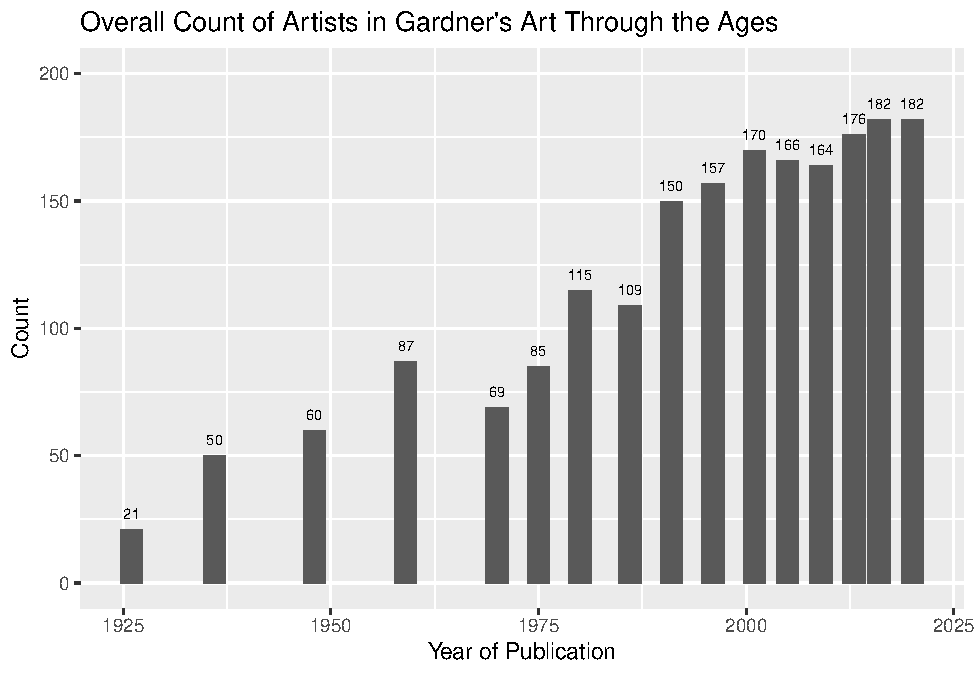
\includegraphics{Chapter1/Chapter1_files/figure-pdf/gardnercountthroughtime-1.pdf}

}

\end{figure}

\begin{verbatim}
# A tibble: 164 x 15
# Groups:   artist_name [164]
   artist_name            edition_number  year artist_national~ artist_national~
   <chr>                           <dbl> <dbl> <chr>            <chr>           
 1 Aaron Douglas                      13  2009 American         American        
 2 Adolphe William Bougu~             13  2009 French           French          
 3 Albert Bierstadt                   13  2009 German-American  Other           
 4 Alfred Stieglitz                   13  2009 American         American        
 5 Ana Mendieta                       13  2009 Cuban-American   Other           
 6 André Derain                       13  2009 French           French          
 7 Andy Warhol                        13  2009 American         American        
 8 Angelica Kauffmann                 13  2009 Swiss            Other           
 9 Anne Louis Girodet Tr~             13  2009 French           French          
10 Anselm Kiefer                      13  2009 German           German          
# ... with 154 more rows, and 10 more variables: artist_gender <chr>,
#   artist_race <chr>, artist_ethnicity <chr>, book <chr>,
#   space_ratio_per_page_total <dbl>, artist_unique_id <int>, moma_count <dbl>,
#   moma_count_to_date <dbl>, whitney_count <dbl>, whitney_count_to_date <dbl>
\end{verbatim}

The shape of the overall count of works by artists in \emph{Gardner's
Art Through the Ages} is heavily left-skewed, multimodal, and
asymmetrical. Such highlights how through time, more works are, on
average, continually added to \emph{Gardner's Art Through the Ages} that
are two-dimensional and made after c.~1750. The first edition, published
in 1926 by Helen Gardner, only has a a total of 21 works. Edition 15,
published in 2016 as well as edition 16, published in 2020, have 182
works respectively, which is the maximum amount of works through all
editions.

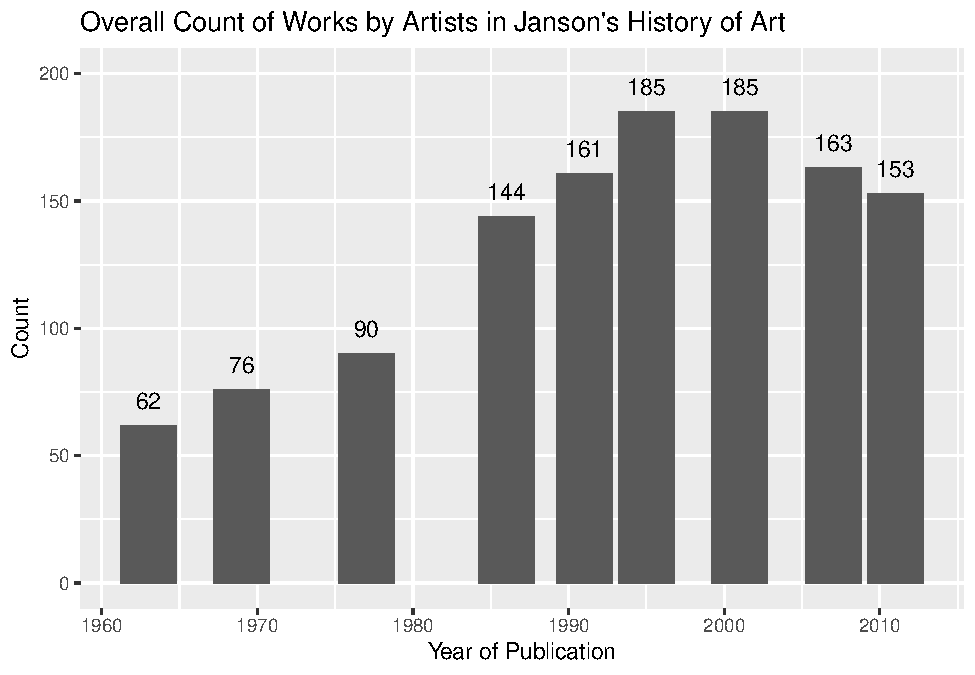
\includegraphics{Chapter1/Chapter1_files/figure-pdf/jansoncountthroughtime-1.pdf}

\begin{verbatim}
# A tibble: 153 x 15
# Groups:   artist_name [153]
   artist_name            edition_number  year artist_national~ artist_national~
   <chr>                           <dbl> <dbl> <chr>            <chr>           
 1 Adolphe William Bougu~              8  2011 French           French          
 2 Albert Pinkham Ryder                8  2011 American         American        
 3 Alexander Rodchenko                 8  2011 Russian          Other           
 4 Alfred Stieglitz                    8  2011 American         American        
 5 Ando Hiroshige                      8  2011 Japanese         Other           
 6 André Derain                        8  2011 French           French          
 7 Andy Warhol                         8  2011 American         American        
 8 Angelica Kauffmann                  8  2011 Swiss            Other           
 9 Anne Louis Girodet Tr~              8  2011 French           French          
10 Anselm Kiefer                       8  2011 German           German          
# ... with 143 more rows, and 10 more variables: artist_gender <chr>,
#   artist_race <chr>, artist_ethnicity <chr>, book <chr>,
#   space_ratio_per_page_total <dbl>, artist_unique_id <int>, moma_count <dbl>,
#   moma_count_to_date <dbl>, whitney_count <dbl>, whitney_count_to_date <dbl>
\end{verbatim}

The shape of the overall count of works by artists in \emph{Janson's
History of Art} is left-skewed, unimodal and asymmetrical. Such
highlights how through time, more works are added to \emph{Janson's
History of Art} that are two-dimensional and made after c.~1750. There
is then a drop-off of works included in the seventh (published in 2007
with 163 works) and eighth (published in 2011 with 153 works) editions,
when new authorship took over. Within edition five (published 1995) and
edition six (published in 2001), both written by Anthony Janson, there
are the same number of works, the maximum amount included in the text
throughout time, 185, as compared to the count of works in the first
edition, first printing, 62, and first edition, second printing, 76.

\hypertarget{gender-through-editions}{%
\section{\texorpdfstring{\textbf{Gender Through
Editions:}}{Gender Through Editions:}}\label{gender-through-editions}}

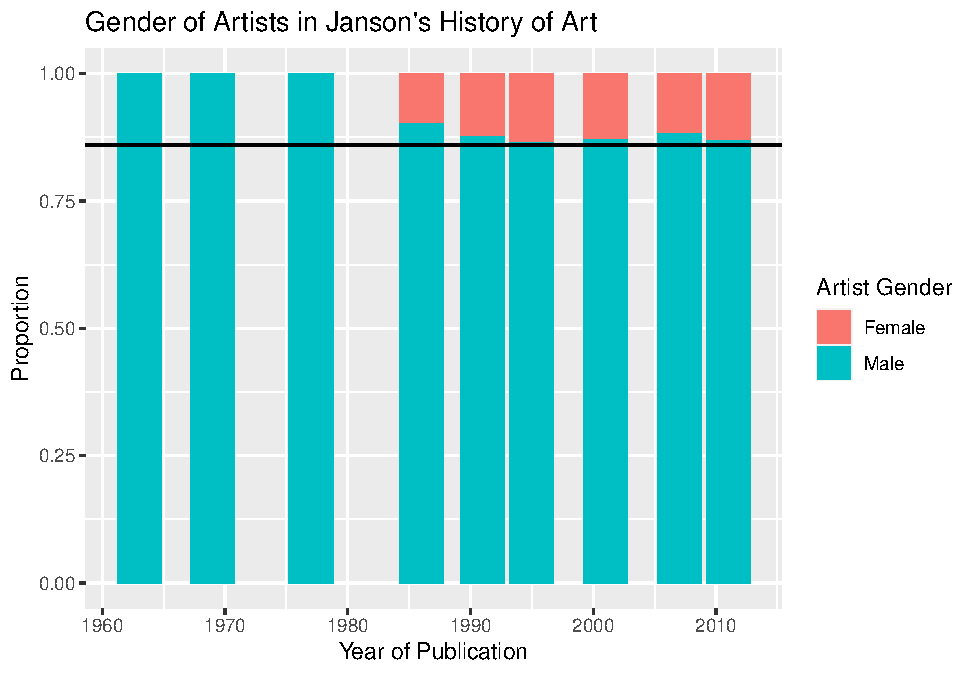
\includegraphics{Chapter1/Chapter1_files/figure-pdf/jansongenderthroughtime-1.pdf}

\begin{verbatim}
[1] 0.899918
\end{verbatim}

The breakdown of artists' gender through editions of \emph{Janson's
History of Art,} has never dipped below 86\% male, which is what the
horizontal line denotes. Additionally, this visualization shows that the
first two editions, (the first three books cataloged: edition 1, first
printing, edition 1, second printing, and edition 2), that were written
my H. W. Janson and Dora Jane Janson, contains no women. Anthony Janson,
who took over authorship for the third edition in 1986, began including
women. Notably, he was extremely proud of himself for diversifying his
family's art history survey text.

The overall percentage of male artists through all books of
\emph{Janson's History of Art} is 89.99\%.

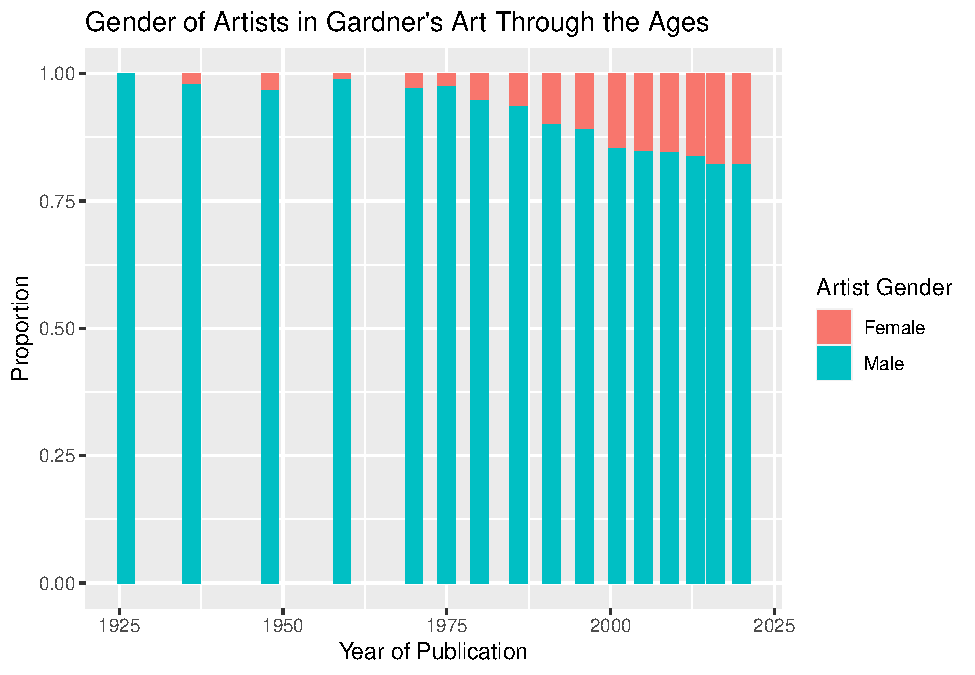
\includegraphics{Chapter1/Chapter1_files/figure-pdf/gardnergenderthroughtime-1.pdf}

\begin{verbatim}
[1] 0.8569223
\end{verbatim}

The breakdown of artists' gender through editions of \emph{Gardner's Art
Through the Ages,} is marginally more diverse in regard to gender, as
the lowest threshold of male artists is just above 81\%, which is
denoted by the horizontal line. Additionally, this visualization shows
that the first edition in 1926 contains no female artists in our scope,
but that starting in the second edition in 1936, Helen Gardner included
female artists.

The overall percentage of male artists through all books of
\emph{Gardner's Art Through the Ages} is 85.69\%, roughly a 4.5\%
increase in regard to gender diversity as compared to \emph{Janson's
History of Art.}

\hypertarget{race-through-editions}{%
\section{\texorpdfstring{\textbf{Race Through
Editions:}}{Race Through Editions:}}\label{race-through-editions}}

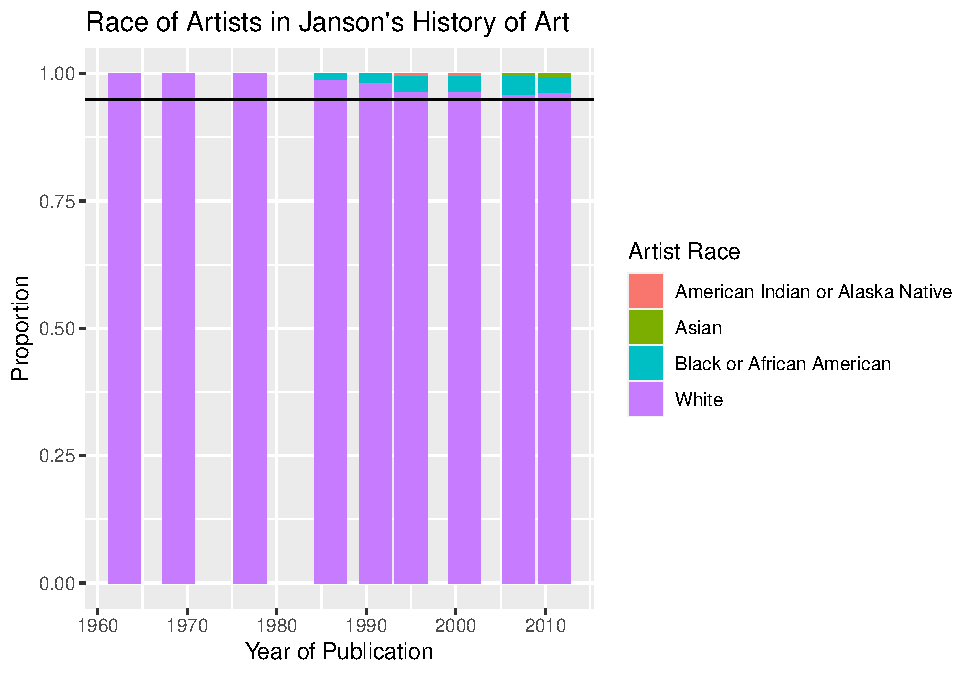
\includegraphics{Chapter1/Chapter1_files/figure-pdf/jansonracethroughtime-1.pdf}

\begin{verbatim}
[1] 0.973749
\end{verbatim}

Pivoting to looking at race diversity in \emph{Janson's History of Art}
through time, unsurprisingly, the three cataloged books, first two
editions written by H. W. Janson and Dora Jane Janson, there were only
white artists included. When their son took over authorship, he included
a handful of black artists, then in the fifth edition, he added an
artist by the name Kay Walkingstick, who is a Native American woman. She
was included through the sixth edition then removed when the group of
six professors took over. Interestingly, the black artists who are
included have frequent turnover. In the seventh and eighth editions,
there was an Asian artist introduced, Ando Hiroshige, a Japanese male
painter who was used as a reference when discussing impressionist art.

The overall percentage of white artists through all editions of
\emph{Janson's History of Art} is 97.37\%.

ADD FIGURE OF WORK USED IN JANSON FOR ANDO HIROSHIGE

\textbf{Figure 1:} Kay WalkingStick, On The Edge, 1989. Acrylic and wax
and oil on canvas, 81 x 162 ½~ cm. Private collection.

\includegraphics{https://lh6.googleusercontent.com/-fxCinylYYA8sB2zbAHmHqqUqxQ26KdZHZgPvNBfgKfWMZqCVK_-VZk2SKqToScRwccJ1ynxTJuI_w2lp0N2BmvgfLPEWl0LO4Ll84ljfkyBkCMQwU8WH-HDC7MXBZpMstMMA8ff.pdf}

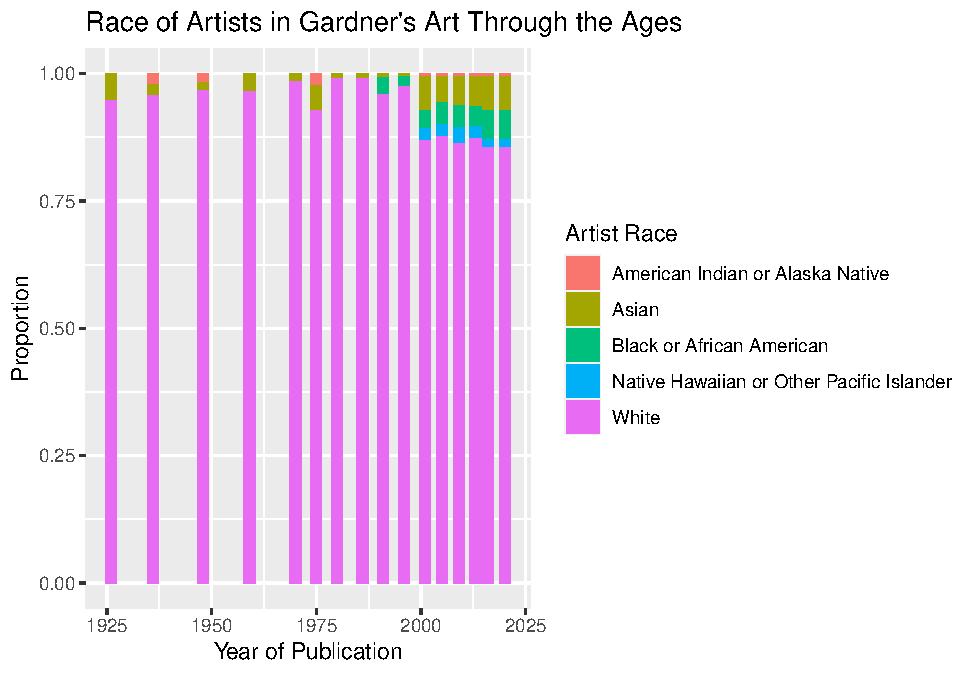
\includegraphics{Chapter1/Chapter1_files/figure-pdf/gardnerracethroughtime-1.pdf}

\begin{verbatim}
[1] 0.9001544
\end{verbatim}

\emph{Gardner's Art Through the Age's} began with including more than
just white artists, with the inclusion of Asian artists in the first
edition. The most diverse a single edition has gotten thus far is just
under 15\% being non-white. Interestingly enough, the two editions that
are least racially diverse are the seventh and eighth editions which
were published in 1980 and 1986 respectively. There is a significant
jump in black representation in the eleventh edition, as well as other
non-white artists as the percentage of non-white artists goes from just
under 4\% in the tenth (1996) to close to 14\% in the eleventh (2001).

The overall percentage of white artists through all editions of
\emph{Gardner's Art Through the Ages} is 90.02\%.

\hypertarget{ethnicity-through-editions}{%
\section{\texorpdfstring{\textbf{Ethnicity Through
Editions:}}{Ethnicity Through Editions:}}\label{ethnicity-through-editions}}

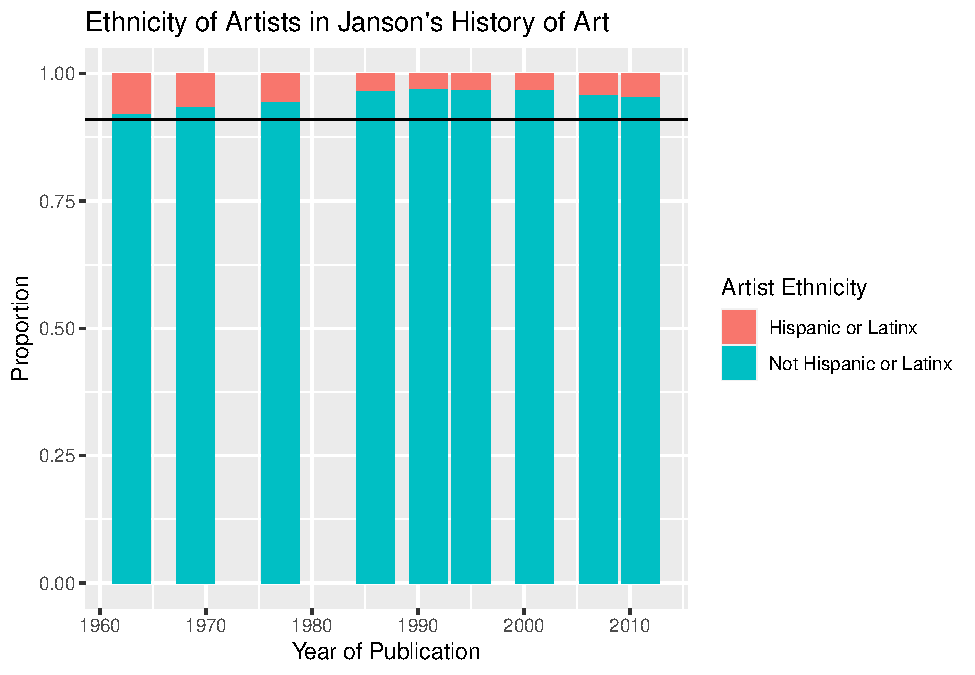
\includegraphics{Chapter1/Chapter1_files/figure-pdf/jansonethnicitythroughtime-1.pdf}

\begin{verbatim}
[1] 0.9581624
\end{verbatim}

Fascinatingly, in \emph{Janson's History of Art,} the ratio of Hispanic
or Latinx artists is the highest of all editions in the first edition,
first printing. This may be because the overall count of artists was so
few that having only a handful of Hispanic or Latinx artists accounted
for just under 9\% of the overall count of artists in the 1963
publication.

The overall percentage of artists who are not Hispanic or Latinx
included in \emph{Janson's History of Art} is 95.82\%.

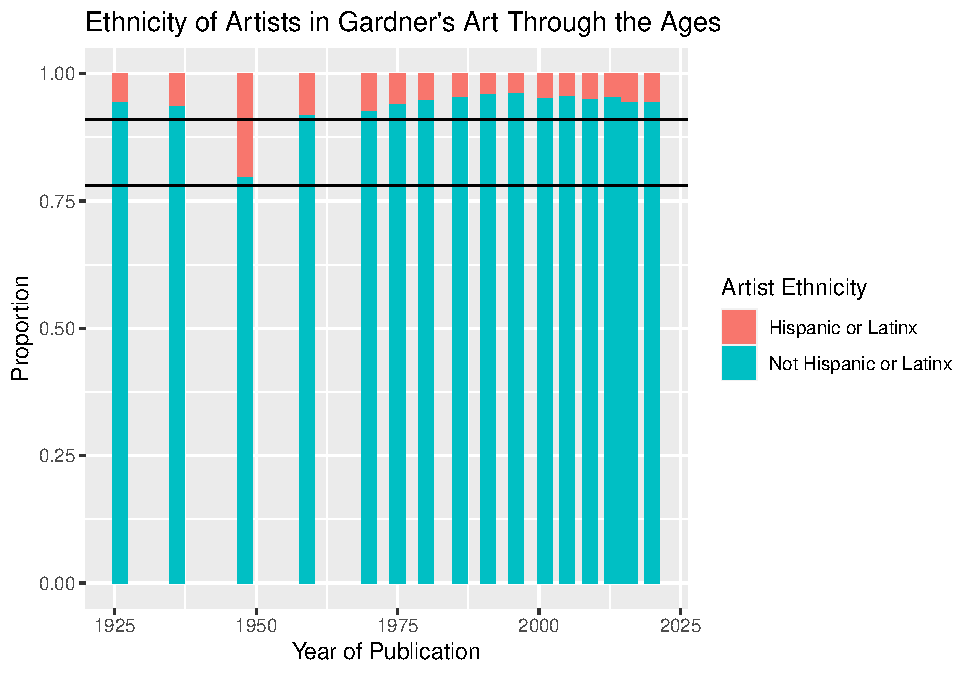
\includegraphics{Chapter1/Chapter1_files/figure-pdf/gardnethnicitythroughtime-1.pdf}

\begin{verbatim}
[1] 0.9150798
\end{verbatim}

Helen Gardner's third edition published in 1959 was the most ethnically
diverse of all 25 textbooks. This edition was published after her death,
but she has passed with the intention of her book being a representation
of the world's history of art. Her efforts are evident through the
percentage of Hispanic and Latinx artists, just under 22\%. It is clear
that her succeeding authors did not continue with such an ethnically
diverse selection of artists, which has remained under 9\% in every
other publication.

The overall percentage of artists who are not Hispanic or Latinx
included in \emph{Janson's History of Art} is 91.51\%.

\hypertarget{nationality-through-editions}{%
\section{\texorpdfstring{\textbf{Nationality Through
Editions:}}{Nationality Through Editions:}}\label{nationality-through-editions}}

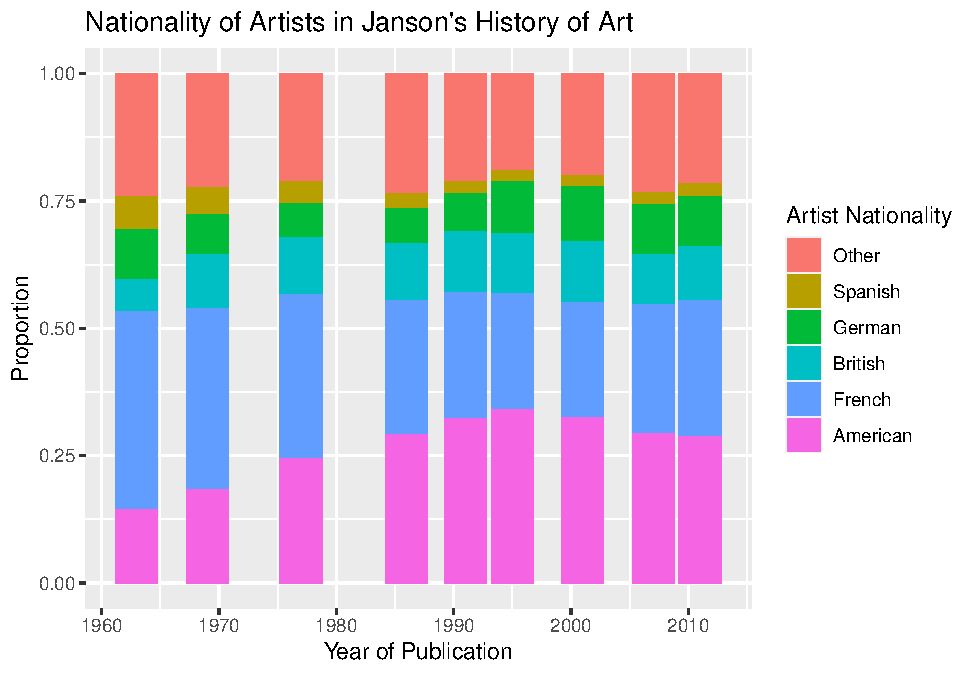
\includegraphics{Chapter1/Chapter1_files/figure-pdf/jansonnationalitythroughtime-1.pdf}

\begin{verbatim}
[1] 0.7850697
\end{verbatim}

It is clear that \emph{Janson's History of Art} paints a western
tradition through the visualization above, highlighting predominantly
French, American, British, German, and Spanish artists. Through the
first two editions---three books as such include the first edition
revised and enlarged published in 1969---the majority nationality is
French. Then, when authorship changes from Peter and Dora Janson to
Anthony F. Janson in the third edition in 1986, the dominant nationality
flips to American. Anthony adds American contemporary artists, such as
Lee Krasner, as well as American photographers such as Dorothea Lange.

The most consistently represented nationality through editions, however,
is French, which could be explained by the type of art highlighted from
after c.~1750: Impressionism, Post-Impressionism and Realism. Artists
such as Édouard Manet and Claude Monet are French painters who enter the
narrative when Peter first writes his discourse published in 1962, and
who remain over time even with change in authorship due to their
perpetual prominence within the art world.

The overall percentage of artists who are French, American, British,
German or Spanish through all editions of \emph{Janson's History of Art}
is 78.51\%.

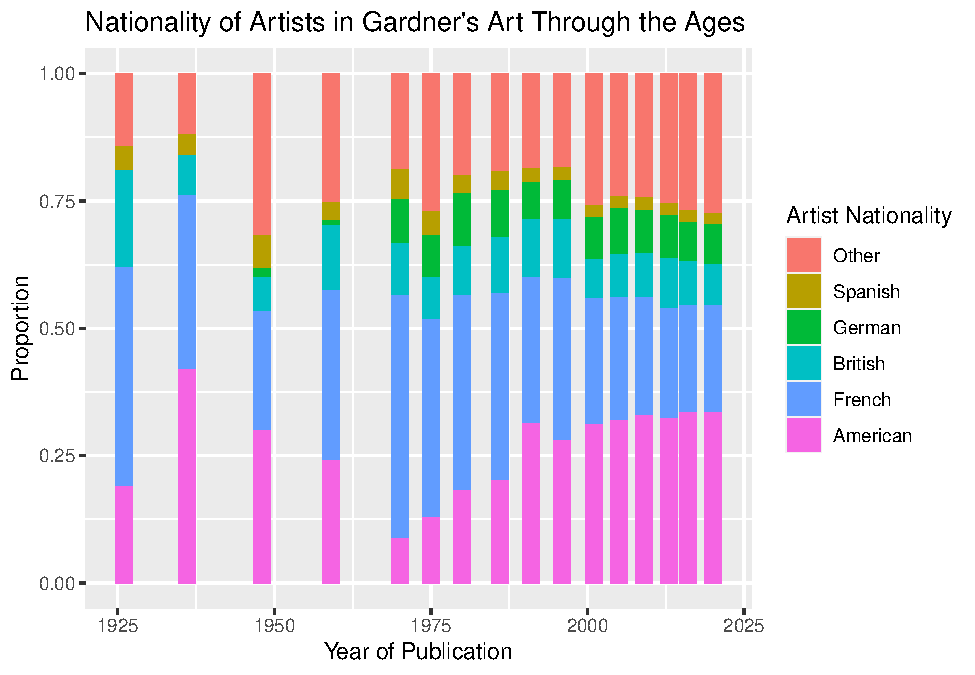
\includegraphics{Chapter1/Chapter1_files/figure-pdf/gardnernationalitythroughtime-1.pdf}

\begin{verbatim}
[1] 0.765826
\end{verbatim}

The spike of the ratio of American artists included in the second
edition published in 1936 could be explained by President Franklin
Delano Roosevelt's Federal Art Project during the Great Depression. The
US government started funding unemployed artists in the US from 1935
through 1943.

This visualization also displays a gradual but significant shift in
dominance from the percentage of French artists included to American
artists from the 1970s through 2020.

The overall percentage of artists who are French, American, British,
German, or Spanish through all editions of \emph{Gardner's Art Through
the Ages} is 76.58\%.

\hypertarget{exploratory-data-analysis-jansons-history-of-art-and-gardners-art-through-the-ages-vs.-total-space-ratio-per-page-per-artist-per-editionspace_ratio_per_page_total}{%
\chapter{\texorpdfstring{Exploratory Data Analysis: \emph{Janson's
History of Art} and \emph{Gardner's Art Through the Ages vs.} Total
Space Ratio per Page per Artist per
Edition\texttt{space\_ratio\_per\_page\_total}}{Exploratory Data Analysis: Janson's History of Art and Gardner's Art Through the Ages vs. Total Space Ratio per Page per Artist per Editionspace\_ratio\_per\_page\_total}}\label{exploratory-data-analysis-jansons-history-of-art-and-gardners-art-through-the-ages-vs.-total-space-ratio-per-page-per-artist-per-editionspace_ratio_per_page_total}}

\hypertarget{distribution-of-space_ratio_per_page_total}{%
\section{\texorpdfstring{Distribution of
\texttt{space\_ratio\_per\_page\_total}}{Distribution of space\_ratio\_per\_page\_total}}\label{distribution-of-space_ratio_per_page_total}}

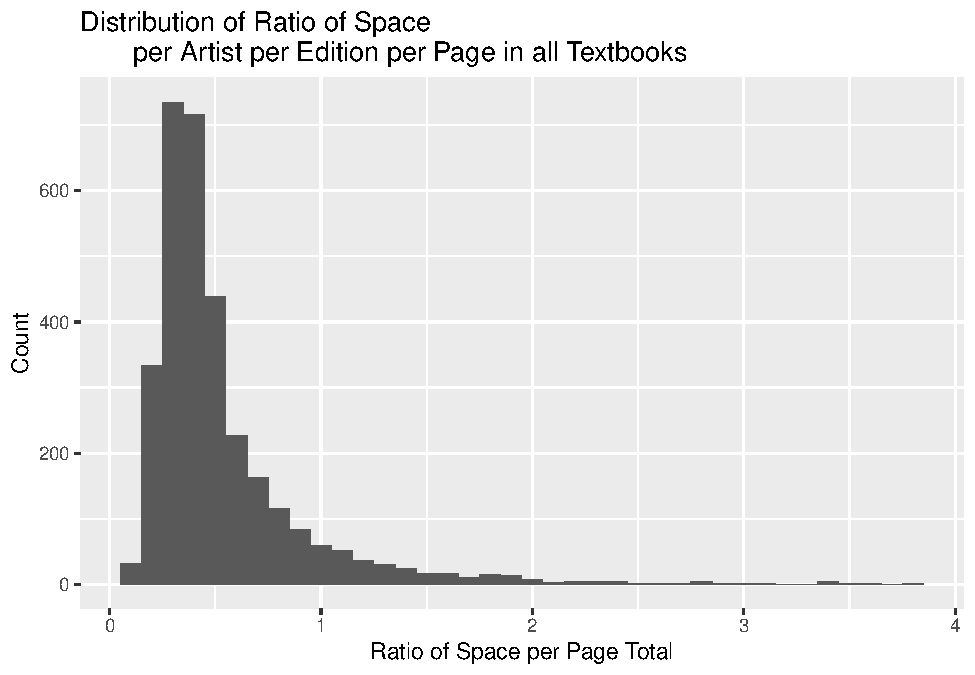
\includegraphics{Chapter1/Chapter1_files/figure-pdf/spaceratioperpagetotal-1.pdf}

\begin{verbatim}
[1] 0.4092838
\end{verbatim}

\begin{verbatim}
[1] 0.2859275
\end{verbatim}

The shape of the visualization above is right-skewed, unimodal and
asymmetrical. Therefore, we would want to look at the median to
understand its center and IQR to understand its spread. The median total
space an artist receives is 40.93\% of a page. The IQR of total space an
artist receives is 28.59\% of a page.

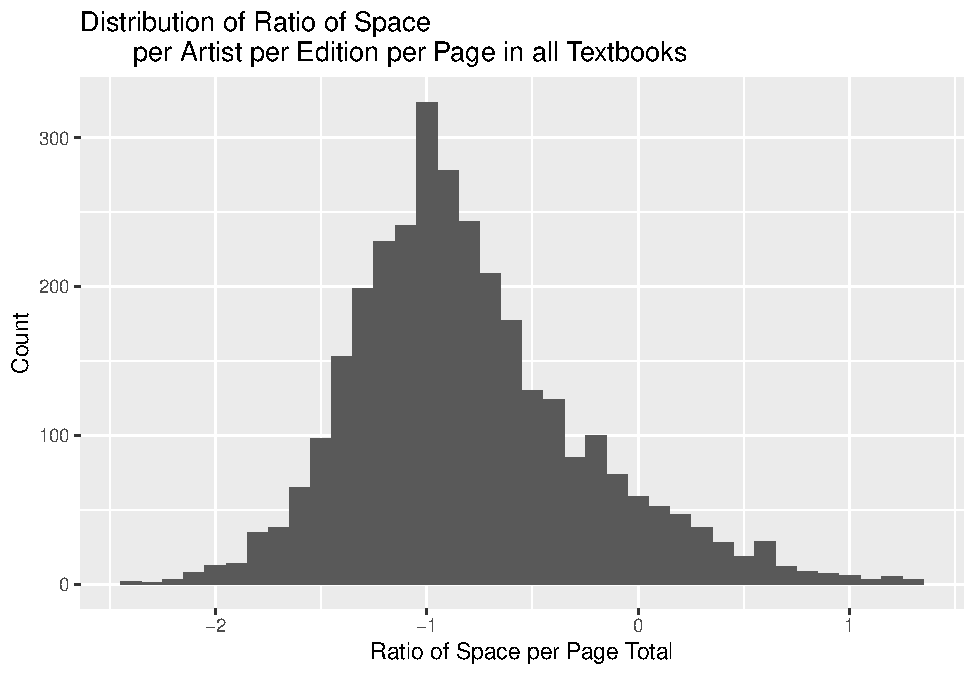
\includegraphics{Chapter1/Chapter1_files/figure-pdf/logspaceratioperpagetotal-1.pdf}

In order to create less skew in our outcome variable, it is evident that
log transforming total space per page given to an artist in a particular
edition gives the spread a much more mild right-skew than before. The
shape is still unimodal and asymmetrical.

\hypertarget{space_ratio_per_page_total-vs.-artist_gender}{%
\section{\texorpdfstring{\texttt{space\_ratio\_per\_page\_total}
vs.~\texttt{artist\_gender}}{space\_ratio\_per\_page\_total vs.~artist\_gender}}\label{space_ratio_per_page_total-vs.-artist_gender}}

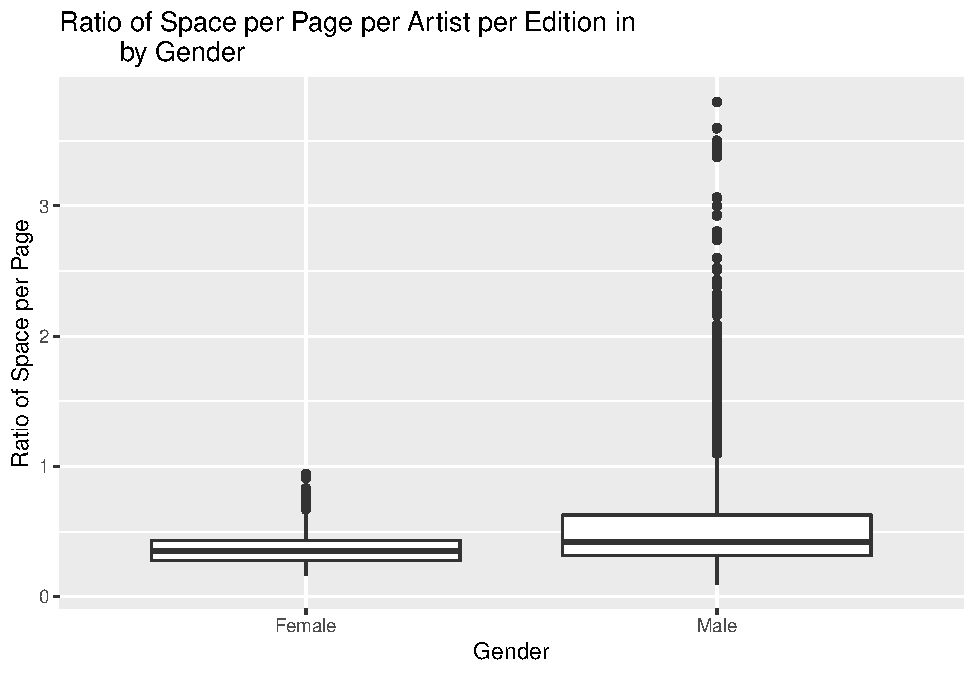
\includegraphics{Chapter1/Chapter1_files/figure-pdf/genderallbooks-1.pdf}

\begin{verbatim}
# A tibble: 10 x 6
# Groups:   artist_name [6]
   artist_name         artist_gender edition_number  year book  space_ratio_per~
   <chr>               <chr>                  <dbl> <dbl> <chr>            <dbl>
 1 Hannah Höch         Female                     8  2011 Jans~            0.940
 2 Hannah Höch         Female                    11  2001 Gard~            0.920
 3 Hannah Höch         Female                     7  2007 Jans~            0.913
 4 Élisabeth Louise V~ Female                    11  2001 Gard~            0.831
 5 Cindy Sherman       Female                    11  2001 Gard~            0.830
 6 Angelica Kauffmann  Female                     8  2011 Jans~            0.797
 7 Liubov Popova       Female                     8  2011 Jans~            0.785
 8 Angelica Kauffmann  Female                    16  2020 Gard~            0.764
 9 Dorothea Rockburne  Female                    10  1996 Gard~            0.736
10 Angelica Kauffmann  Female                     7  2007 Jans~            0.733
\end{verbatim}

\begin{verbatim}
[1] 0.3492886
\end{verbatim}

\begin{verbatim}
[1] 0.4202227
\end{verbatim}

\begin{verbatim}
[1] 0.1081594
\end{verbatim}

Interestingly enough, the median of the total ratio of space per page
for female artists is 0.349, not far below the median of the total ratio
of space per page in centimeters for male artists, 0.42 through all 25
varying textbooks\emph{.} This indicates that even though the percentage
of female artists as compared to male artists is 10.82\%, the average
amount of space allotted to a female artist is comparable to that of a
male.

That said, there are far more male artists that are given a total ratio
of space per page of over 1, meaning over a page of information
regarding their work or works. No female has a total ratio of space per
page of over 1. The closest female artist to having a page of area given
to them is Hannah Höch. In fact, she holds the top three spots of the
most area given to a woman in three separate editions: The seventh
(2007) and eighth (2011) editions of \emph{Janson's History of Art} and
the eleventh edition (2001) of \emph{Gardner's Art Through the Ages.}

LOOK AT WHICH WORK OF HERS IS INCLUDED IN EACH EDITION.

\hypertarget{space_ratio_per_page_total-vs.-artist_race}{%
\section{\texorpdfstring{\texttt{space\_ratio\_per\_page\_total}
vs.~\texttt{artist\_race}}{space\_ratio\_per\_page\_total vs.~artist\_race}}\label{space_ratio_per_page_total-vs.-artist_race}}

The median of the total ratio of space given to a particular artist
through all 25 books is fairly comparable across varying races. Though
the count of each race is far from being comparable, the respective
medians per race are as follows: American Indian or Alaska Native, .469,
Asian, .344, Black or African American .375, Native Hawaiian or Other
Pacific Islander, .428 and White, .413. With that being said, even
though the racial diversity in regard to the ratio of count for white to
non-white artists is 92.85\%, once an artist is represented, the amount
of area given to them is fairly similar in regard to their respectively
medians.

Obviously, the top quartile of white artists dominates this
visualization. White is the only race that has any artists given more
than a page of space in any one book. Out of the top ten outliers of
white artists, eight of them are Pablo Picasso, with the first five
observations being from various editions of \emph{Janson's History of
Art.}

\hypertarget{space_ratio_per_page_total-vs.-artist_ethnicity}{%
\section{\texorpdfstring{\texttt{space\_ratio\_per\_page\_total}
vs.~\texttt{artist\_ethnicity}}{space\_ratio\_per\_page\_total vs.~artist\_ethnicity}}\label{space_ratio_per_page_total-vs.-artist_ethnicity}}

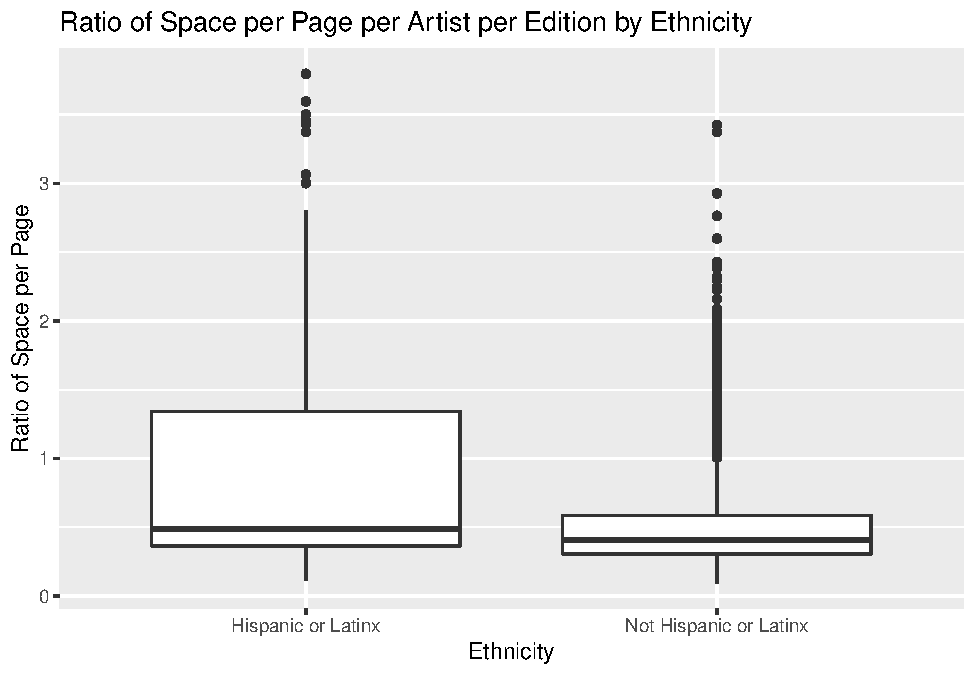
\includegraphics{Chapter1/Chapter1_files/figure-pdf/ethnicityallbooks-1.pdf}

\begin{verbatim}
[1] 0.4879276
\end{verbatim}

\begin{verbatim}
[1] 0.4060381
\end{verbatim}

Interestingly, the median \texttt{space\_ratio\_per\_page\_total} for
artists who are Hispanic or Latinx,
\texttt{round(median(janson\_HL\$space\_ratio\_per\_page\_total),\ 3)}
is higher than those who are Not Hispanic or Latinx,
\texttt{round(median(janson\_NHL\$space\_ratio\_per\_page\_total),\ 3)}.
There are \texttt{nrow(janson\_HL)} observations of artists per edition
who are Hispanic and Latinx and there are \texttt{nrow(janson\_NHL)}
observations of artists per edition who are not Hispanic or Latinx.
Picasso plays a large role in such, as he is Hispanic or Latinx and is
accounting for the outlyingly larger observations for
\texttt{space\_ratio\_per\_page\_total}.

\hypertarget{space_ratio_per_page_total-vs.-artist_nationality_other}{%
\section{\texorpdfstring{\texttt{space\_ratio\_per\_page\_total}
vs.~\texttt{artist\_nationality\_other}}{space\_ratio\_per\_page\_total vs.~artist\_nationality\_other}}\label{space_ratio_per_page_total-vs.-artist_nationality_other}}

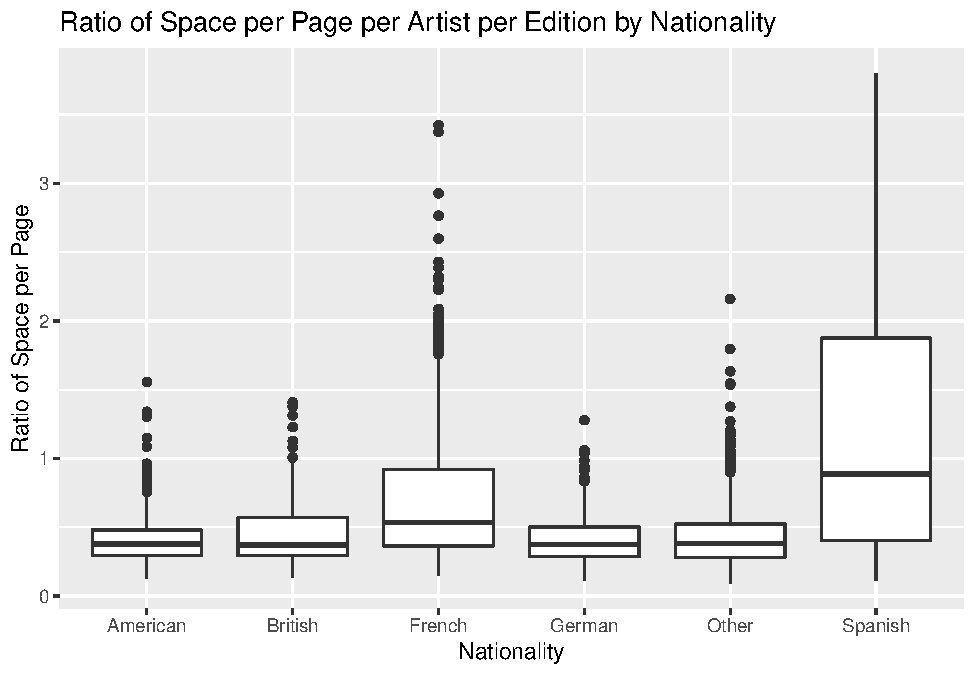
\includegraphics{Chapter1/Chapter1_files/figure-pdf/nationalityotherallbooks-1.pdf}

\hypertarget{section}{%
\section{}\label{section}}

\hypertarget{model-exploration}{%
\chapter{Model Exploration}\label{model-exploration}}

\hypertarget{data-preparation-for-modeling}{%
\chapter{Data Preparation for
Modeling:}\label{data-preparation-for-modeling}}

\begin{verbatim}
# A tibble: 6 x 2
  artist_nationality_other     n
  <fct>                    <int>
1 American                   896
2 French                     870
3 Other                      671
4 British                    317
5 German                     256
6 Spanish                     94
\end{verbatim}

\hypertarget{model-exploration-1}{%
\chapter{Model Exploration:}\label{model-exploration-1}}

\begin{verbatim}
ddf="Satterthwaite"
\end{verbatim}

Satterthwaite test, more flexible, looking directly at p-values -
non-parametric test - uses different error term, similar to a two same
t-test, similar to ANOVA - analysis of variance - checking between
different groups -

\begin{verbatim}
Backward reduced random-effect table:

                  Eliminated npar  logLik    AIC    LRT Df Pr(>Chisq)    
<none>                         23 -1930.6 3907.2                         
(1 | artist_name)          0   22 -2606.4 5256.9 1351.7  1  < 2.2e-16 ***
---
Signif. codes:  0 '***' 0.001 '**' 0.01 '*' 0.05 '.' 0.1 ' ' 1

Backward reduced fixed-effect table:
Degrees of freedom method: Satterthwaite 

                                            Eliminated Sum Sq Mean Sq NumDF
artist_race_nwi:moma_count_to_date                   1 0.0015 0.00151     1
artist_ethnicity:whitney_count_to_date               2 0.0092 0.00922     1
artist_ethnicity:moma_count_to_date                  3 0.1130 0.11296     1
artist_ethnicity                                     4 0.0057 0.00574     1
artist_gender                                        5 0.3801 0.19006     2
artist_race_nwi:whitney_count_to_date                6 0.1548 0.15478     1
whitney_count_to_date                                7 0.0232 0.02319     1
artist_race_nwi                                      8 0.0426 0.04263     1
artist_nationality_other:moma_count_to_date          0 3.3446 0.66892     5
                                              DenDF F value   Pr(>F)   
artist_race_nwi:moma_count_to_date           539.28  0.0091 0.923923   
artist_ethnicity:whitney_count_to_date      1970.66  0.0559 0.813065   
artist_ethnicity:moma_count_to_date          731.38  0.6850 0.408150   
artist_ethnicity                             505.76  0.0348 0.852153   
artist_gender                                401.31  1.1522 0.316977   
artist_race_nwi:whitney_count_to_date        480.27  0.9384 0.333175   
whitney_count_to_date                        984.87  0.1406 0.707781   
artist_race_nwi                              510.52  0.2585 0.611386   
artist_nationality_other:moma_count_to_date 1221.63  4.0556 0.001178 **
---
Signif. codes:  0 '***' 0.001 '**' 0.01 '*' 0.05 '.' 0.1 ' ' 1

Model found:
log(space_ratio_per_page_total) ~ artist_nationality_other + moma_count_to_date + (1 | artist_name) + artist_nationality_other:moma_count_to_date
\end{verbatim}

pick a handful of interest

visualization : confidence intervals for each on of the slopes

predictors on the y axis -

bar plots of the pvalues another option

nationality discourse for significance

log transformation on the y variable -

stepwise model selection

the multiple of the number of degrees of freedom used for the penalty.
Only k = 2 gives the genuine AIC: k = log(n) is sometimes referred to as
BIC or SBC.

\begin{verbatim}
Linear mixed model fit by maximum likelihood . t-tests use Satterthwaite's
  method [lmerModLmerTest]
Formula: log(space_ratio_per_page_total) ~ artist_nationality_other +  
    moma_count_to_date + artist_nationality_other * moma_count_to_date +  
    (1 | artist_name)
   Data: gardnerjanson_museums

     AIC      BIC   logLik deviance df.resid 
  3893.6   3978.2  -1932.8   3865.6     3090 

Scaled residuals: 
    Min      1Q  Median      3Q     Max 
-3.6304 -0.5820 -0.0716  0.6203  3.0709 

Random effects:
 Groups      Name        Variance Std.Dev.
 artist_name (Intercept) 0.1274   0.3569  
 Residual                0.1649   0.4061  
Number of obs: 3104, groups:  artist_name, 395

Fixed effects:
                                                     Estimate Std. Error
(Intercept)                                        -9.291e-01  4.017e-02
artist_nationality_otherFrench                      2.681e-01  6.377e-02
artist_nationality_otherOther                      -6.192e-02  5.836e-02
artist_nationality_otherBritish                     1.044e-02  8.093e-02
artist_nationality_otherGerman                     -6.204e-02  8.653e-02
artist_nationality_otherSpanish                     6.589e-01  2.002e-01
moma_count_to_date                                 -1.026e-02  6.948e-03
artist_nationality_otherFrench:moma_count_to_date   2.872e-02  7.962e-03
artist_nationality_otherOther:moma_count_to_date    1.580e-02  8.077e-03
artist_nationality_otherBritish:moma_count_to_date  1.011e-02  1.689e-02
artist_nationality_otherGerman:moma_count_to_date   2.433e-02  8.943e-03
artist_nationality_otherSpanish:moma_count_to_date  3.528e-02  9.481e-03
                                                           df t value Pr(>|t|)
(Intercept)                                         4.979e+02 -23.131  < 2e-16
artist_nationality_otherFrench                      4.367e+02   4.205 3.17e-05
artist_nationality_otherOther                       5.139e+02  -1.061 0.289240
artist_nationality_otherBritish                     4.405e+02   0.129 0.897407
artist_nationality_otherGerman                      4.758e+02  -0.717 0.473735
artist_nationality_otherSpanish                     3.689e+02   3.291 0.001096
moma_count_to_date                                  8.440e+02  -1.477 0.140001
artist_nationality_otherFrench:moma_count_to_date   1.037e+03   3.607 0.000324
artist_nationality_otherOther:moma_count_to_date    8.326e+02   1.956 0.050764
artist_nationality_otherBritish:moma_count_to_date  7.812e+02   0.599 0.549598
artist_nationality_otherGerman:moma_count_to_date   1.031e+03   2.721 0.006617
artist_nationality_otherSpanish:moma_count_to_date  1.819e+03   3.721 0.000205
                                                      
(Intercept)                                        ***
artist_nationality_otherFrench                     ***
artist_nationality_otherOther                         
artist_nationality_otherBritish                       
artist_nationality_otherGerman                        
artist_nationality_otherSpanish                    ** 
moma_count_to_date                                    
artist_nationality_otherFrench:moma_count_to_date  ***
artist_nationality_otherOther:moma_count_to_date   .  
artist_nationality_otherBritish:moma_count_to_date    
artist_nationality_otherGerman:moma_count_to_date  ** 
artist_nationality_otherSpanish:moma_count_to_date ***
---
Signif. codes:  0 '***' 0.001 '**' 0.01 '*' 0.05 '.' 0.1 ' ' 1

Correlation of Fixed Effects:
            (Intr) art__F art__O art__B art__G art__S mm_c__ a__F:_ a__O:_
artst_ntn_F -0.630                                                        
artst_ntn_O -0.688  0.434                                                 
artst_ntn_B -0.496  0.313  0.342                                          
artst_ntn_G -0.464  0.292  0.319  0.230                                   
artst_ntn_S -0.201  0.126  0.138  0.100  0.093                            
mm_cnt_t_dt -0.458  0.288  0.315  0.227  0.213  0.092                     
arts__F:___  0.400 -0.356 -0.275 -0.198 -0.185 -0.080 -0.873              
arts__O:___  0.394 -0.248 -0.399 -0.195 -0.183 -0.079 -0.860  0.751       
arts__B:___  0.188 -0.119 -0.130 -0.366 -0.087 -0.038 -0.411  0.359  0.354
arts__G:___  0.356 -0.224 -0.245 -0.177 -0.349 -0.071 -0.777  0.678  0.668
arts__S:___  0.336 -0.211 -0.231 -0.167 -0.156 -0.305 -0.733  0.640  0.630
            a__B:_ a__G:_
artst_ntn_F              
artst_ntn_O              
artst_ntn_B              
artst_ntn_G              
artst_ntn_S              
mm_cnt_t_dt              
arts__F:___              
arts__O:___              
arts__B:___              
arts__G:___  0.320       
arts__S:___  0.302  0.569
\end{verbatim}

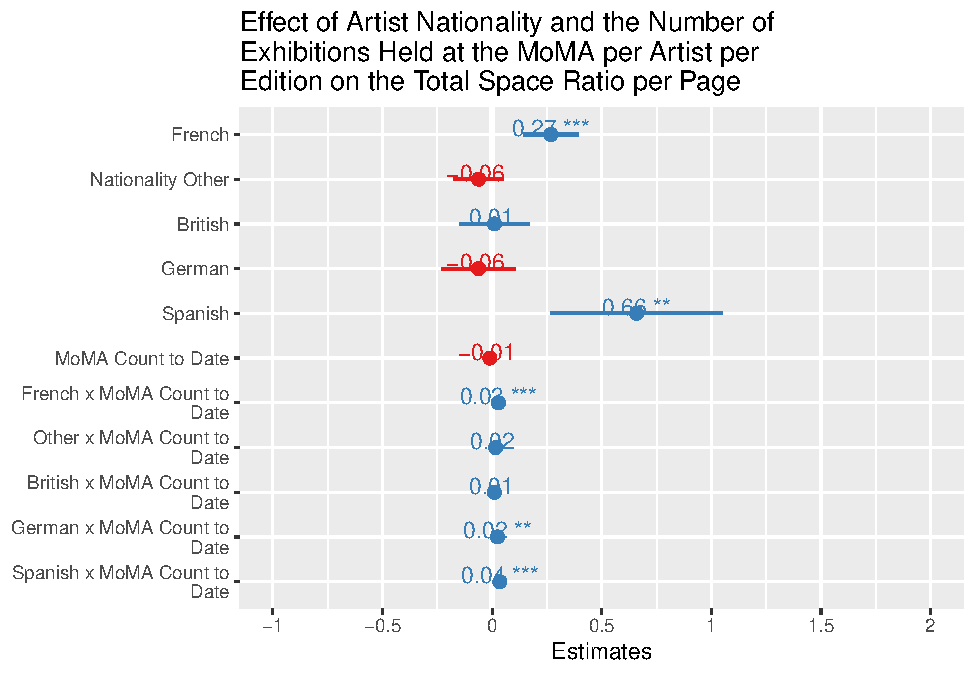
\includegraphics{Chapter2/Chapter2_files/figure-pdf/sjplot-1.pdf}

\begin{verbatim}
                                                GVIF Df GVIF^(1/(2*Df))
artist_nationality_other                     1.94725  5        1.068913
moma_count_to_date                          10.07286  1        3.173778
artist_nationality_other:moma_count_to_date 16.54427  5        1.323929
\end{verbatim}

GET PVALUES FOR COEFFICIENTS - STATISTICALLY SIGNIFICANT - GO THROUGH
INTERPRETATIONS WITH LOG TRANSFORMATION AND MIXED EFFECTS MODEL -
CONFIRM MODEL DIAGNOSTICS - AIC / BIC FOR MIXED EFFECTS -

\begin{verbatim}
          R2m       R2c
[1,] 0.171159 0.5323004
\end{verbatim}

Marginal R2 provides the variance explained only by fixed effects and
conditional R2 provides the variance explained by the entire model,
i.e., both fixed effects and random effects.

Model Diagnostics : Check for linearity, independence, residuals, normal
distribution of the residuals - no pattern in residuals, constant
variance

RESOURCE: https://www.ssc.wisc.edu/sscc/pubs/MM/MM\_DiagInfer.html

Plotting : log transform some variables : Fitted v. Residuals

\hypertarget{appendix}{%
\chapter{Appendix:}\label{appendix}}

\hypertarget{assumptions}{%
\section{Assumptions:}\label{assumptions}}

\hypertarget{residuals-and-constant-variance}{%
\subsection{Residuals and Constant
Variance:}\label{residuals-and-constant-variance}}

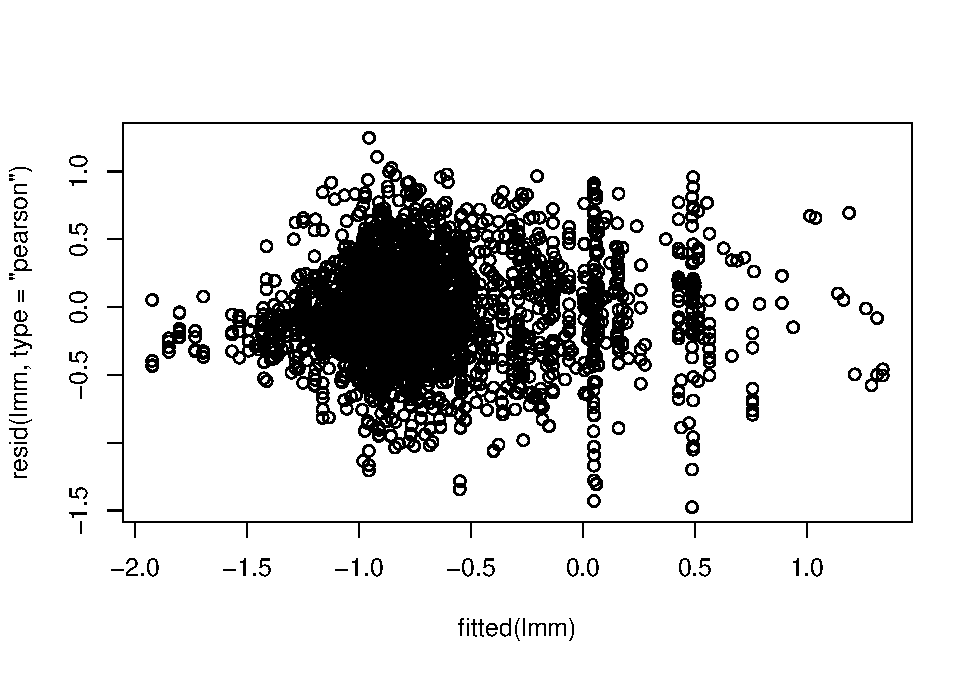
\includegraphics{Chapter2/Chapter2_files/figure-pdf/diagnostics-1.pdf}

for the very low values of the predicted have very low variability for
residuals - the rest varied

the a bulk of the data there is constant variability in the residuals

before log transforming our outcome variable, the constant variance
assumption was violated. Therefore, in order to pass the constant
variance assumption, I performed a log transformation.

\hypertarget{normality}{%
\subsection{Normality:}\label{normality}}

normal histogram = density plot overlayed -

Struggling to understand how to do this with a mixed-effects model

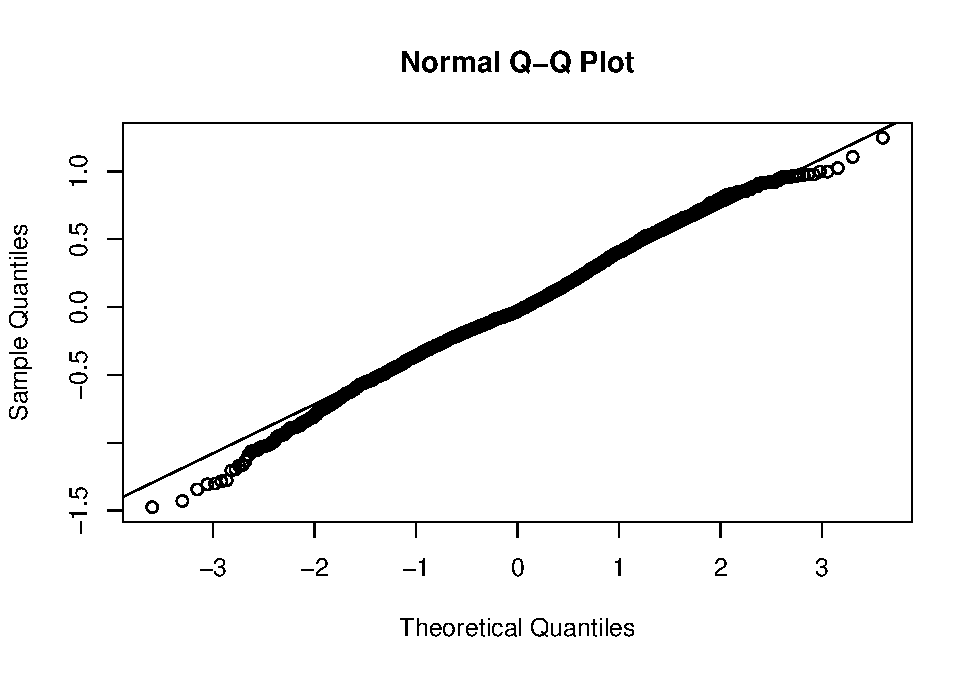
\includegraphics{Chapter2/Chapter2_files/figure-pdf/normal-1.pdf}

\hypertarget{linearity}{%
\subsection{Linearity:}\label{linearity}}

residuals v quantitative predictors

once i figure out how to augment the data and get the .resid I can make
this visualization as well

no pattern is left behind

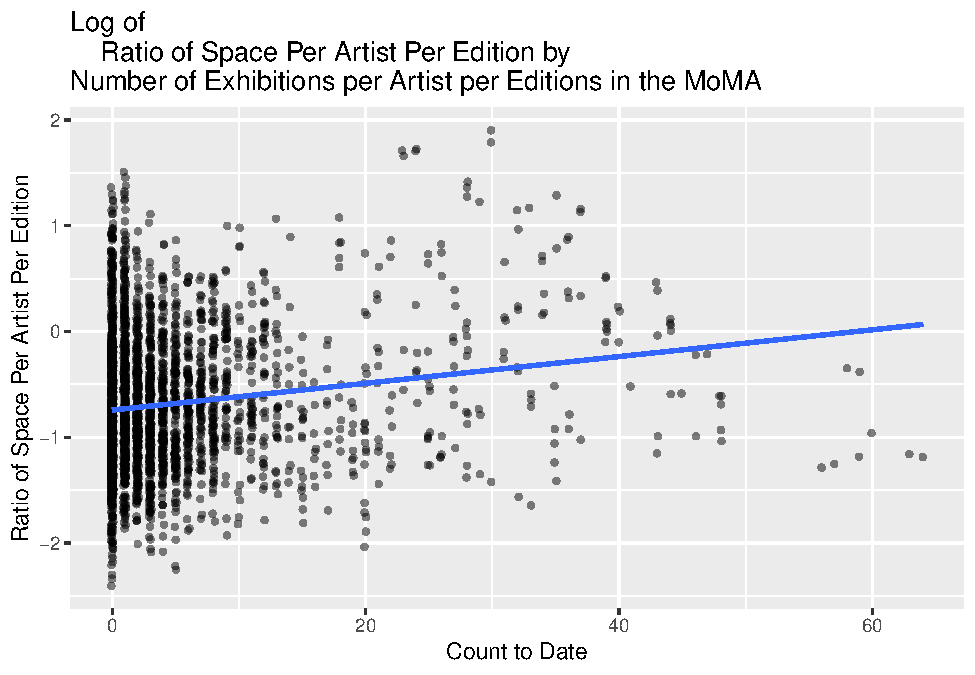
\includegraphics{Chapter2/Chapter2_files/figure-pdf/linearitymoma-1.pdf}

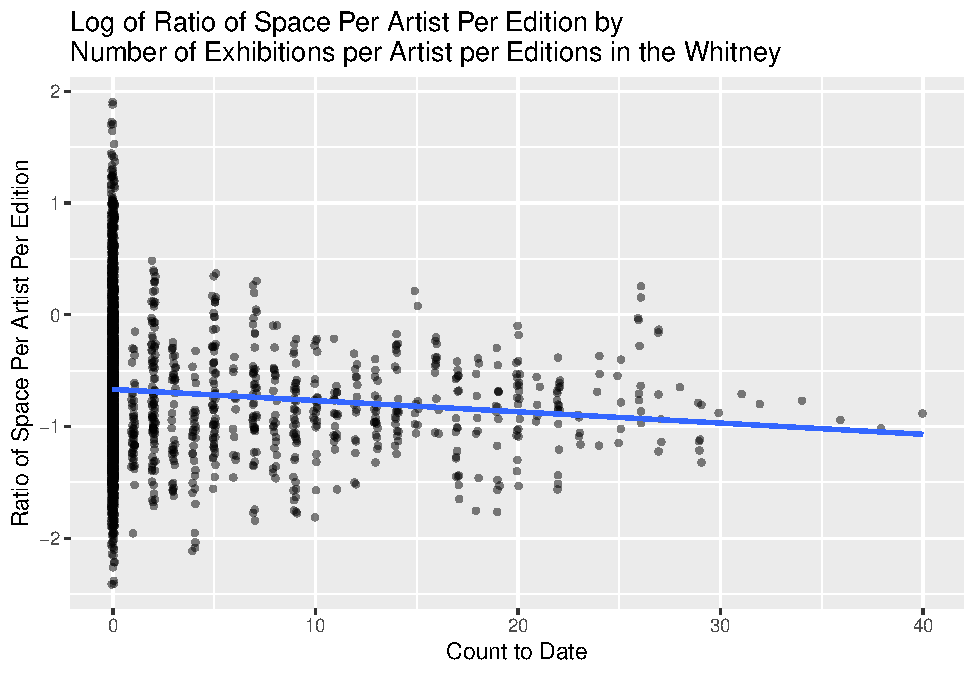
\includegraphics{Chapter2/Chapter2_files/figure-pdf/linearitywhitney-1.pdf}

Normality of random effect: Get the estimate of random effect (in your
case random intercepts), and check them as check the residual. But it is
not efficient because you just have 7 random intercepts.

\hypertarget{independence}{%
\subsection{Independence:}\label{independence}}

Another assumption is the independence between subjects. No test, based
on your judgement. Subject specific random intercept means the
correlation between the response variable from the same subject are the
same.

all obervations of different artists are independent -

fitting a mixed model - i do not believe that pieces by each artist is
independence - at the artist level we have independence

log transforming predictors - interpretations change - variables weren't
changed - same idea, bit different

INDEPENDENCE: DOUBLE CHECK - EMPIRICALLY ARGUE OR ?

check for time series - residuals v. order of data points

irrelevant - based on how the sample was collected.

verbally argue the independence between artists - since we are using a
mixed effects model, and our random effect is per artist, we eliminate
the dependence of our observations had we not used a mixed effects
model. Between artists, we expect the observations to be independent.

\hypertarget{data-dictionary}{%
\section{\texorpdfstring{\textbf{Data
Dictionary:}}{Data Dictionary:}}\label{data-dictionary}}

Outcome:

\texttt{space\_ratio\_per\_page\_total} = The area in centimeters
squared of both the text and the figure of a particular artist in a
given edition of \emph{Janson's History of Art} divided by the area in
centimeters squared of a single page of the respective edition.

Potential Predictors:

\texttt{artist\_gender} = The gender of the artist.

\texttt{artist\_race} = The race of the artist.

\texttt{artist\_race\_nwi} = The non-white indicator for artist race,
meaning if an artist's race is denoted as either white or non-white.

\texttt{artist\_ethnicity} = The ethnicity of the artist.

\texttt{artist\_nationality\_other} = The nationality of the artist.
Roughly 80\% of of the total count of artists through all editions of
Janson account for French, Spanish, British, American and German.
Therefore, the categorical strings of this variable are French, Spanish,
British, American, German and Other.

\texttt{whitney\_count\_to\_date} = The count of exhibitions held by The
Whitney of a particular artist at a particular moment of time, as
highlighted by \texttt{year}.

\texttt{moma\_count\_to\_date} = The count of exhibitions held by the
Museum of Modern Art (MoMA) of a particular artist at a particular
moment of time, as highlighted by \texttt{year}.

\texttt{year} = The year of publication for a given edition of Janson or
Gardner.

Other variables:

\texttt{edition\_number} = The edition number of the textbook from
either Janson's History of Art or Gardner's Art Through the Ages.

\texttt{book} = Which book, either Janson or Gardner the particular
artist at that particular time was included.

\texttt{artist\_unique\_id} = A unique identifying number assigned to
artists across books and editions denoted in alphabetical order.

\end{document}
